%  The following commands have been added in the SPIE class 
%  file (spieman.cls) and may not be understood in other classes:
%  \affiliations{}, \sup{},\supit{}, \authorinfo{}, \keywords{},
%  \linkable and \video
%  The bibliography style file is called spiejour.bst 

\documentclass[12pt]{spieman}  %>>> 12pt font mandatory; use this for US letter paper 
%%\documentclass[a4paper,12pt]{spieman}  %>>> use this instead for A4 paper
%%\documentclass[nocompress,12pt]{spieman}  %>>> to avoid compression of citations
%% \addtolength{\voffset}{9mm}   %>>> moves text field down
 
\usepackage[]{graphicx}
\usepackage{setspace}
\usepackage{tocloft}
\usepackage{units}
\usepackage{nicefrac}
\usepackage{color}
\usepackage{epstopdf}
\usepackage[globalcitecopy,labelstoglobalaux,sectionbib]{bibunits}
\usepackage[thinspace,thinqspace,squaren]{SIunits}
\usepackage{fancyhdr}
\usepackage{url}
\usepackage{wasysym}
%\usepackage{alltt}
%\renewcommand{\ttdefault}{txtt} 
\usepackage{array}
%\usepackage[version=3]{mhchem}
%\usepackage[T1]{fontenc}
%\usepackage{textcomp}
%\usepackage{verbatim} 
%\usepackage{mathpazo}
%\usepackage{amsmath} %>>> for AMS math formatting including bold Greek symbols
%\usepackage{mathtools}
\usepackage{amssymb}
\usepackage{accents}
%\usepackage{hyperref}
\usepackage{url}
\usepackage{amscd}
\usepackage{epsfig}
\usepackage{cite}
\usepackage{subfig}
\usepackage[globalcitecopy,labelstoglobalaux,sectionbib]{bibunits}
%\usepackage[sectionbib]{bibunits}
\usepackage{appendix}
\usepackage{slashbox}
\usepackage{multirow}
\usepackage{pbox}
%\usepackage{caption}
\usepackage{pdflscape}
\usepackage{nicefrac}
\usepackage{rotating}
\usepackage[colorlinks=true,citecolor=blue,urlcolor=blue,linkcolor=blue,
		pagebackref,
		hyperindex,%linktocpage,
		bookmarksnumbered=true,bookmarksopen=true,bookmarksopenlevel=0,
		pdfstartview=FitV,
		pdfstartpage=1]
	{hyperref} % makes pdf look nice with hyperlinks

\title{Comprehensive optical and data management infrastructure for high-throughput light-sheet microscopy of whole mouse brains} 

\author{M. Caroline M\"{u}llenbroich,\supscr{a,b} Ludovico Silvestri, \supscr{a,c} Leonardo Onofri,\supscr{e} Irene Costantini,\supscr{a} Marcel van 't Hoff,\supscr{a,b} Leonardo Sacconi,\supscr{a,c} Giulio Iannello,\supscr{e} Francesco S. Pavone,\supscr{a,b,c,d}  }

\affiliation{\supscrsm{a}European Laboratory for Non-linear Spectroscopy (LENS), University of Florence, Italy\\
\supscrsm{b}Department of Physics and Astronomy, University of Florence, Italy\\
\supscrsm{c}National Institute of Optics, National Research Council, Italy\\
\supscrsm{d}International Center for Computational Neurophotonics (ICON Foundation), Italy\\
\supscrsm{e}Integrated Research Centre, University Campus Bio-Medico of Rome, Italy\\
%\supscrsm{f}Distrio, Amsterdam, The Netherlands
}

%%%%%%%%%%%%%%%%%%%%%%%%%%%%%%%%%%%%%%%%%%%%%%%%%%%%%%%%%%%%% 
\renewcommand{\cftdotsep}{\cftnodots}
\cftpagenumbersoff{figure}
\cftpagenumbersoff{table} 
\begin{document} 
\maketitle 

%%%%%%%%%%%%%%%%%%%%%%%%%%%%%%%%%%%%%%%%%%%%%%%%%%%%%%%%%%%%% 
\begin{abstract}
The comprehensive mapping and quantification of neuronal projections in the central nervous system requires high-throughput imaging of large volumes with microscopic resolution. We have developed a confocal light-sheet microscope that has been optimised for the 3D imaging of structurally intact clarified whole-mount mouse brains. Here we describe the optical and electro-mechanical arrangement of the microscope and give details on the organisation of the microscope management software. The software orchestrates all components of the microscope, coordinates critical timing and synchronisation and has been written in a versatile and modular structure using the LabVIEW language.  It can easily be adapted and integrated to other microscope systems and has been made freely available to the light-sheet community. The tremendous amount of data routinely generated by light-sheet microscopy further requires novel strategies for data handling and storage. To complete the full imaging pipeline of our high- throughput microscope we further elaborate on big data management from the data streaming of raw images up to stitching and visualisation of 3D data sets. The meso-scale neuroanatomy imaged at micron-scale resolution in those datasets allows characterization and quantification of neuronal projections in unsectioned mouse brains. 
\end{abstract}

%>>>> Include a list of up to six keywords after the abstract
\keywords{Light-sheet microscopy, whole brain mounting, whole brain imaging, big data, data management, software management, imaging pipeline, high-throughput imaging}

%>>>> Include contact information for corresponding author
{\noindent \footnotesize{\bf Address all correspondence to}: First author, University Name, Faculty Group, Department, Street Address, City, Country, Postal Code; Tel: +1 555-555-5555; Fax: +1 555-555-5556; E-mail:  \linkable{myemail@university.edu} }
%%%%%%%%%%%%%%%%%%%%%%%%%%%%%%%%%%%%%%%%%%%%%%%%%%%%%%%%%%%%%

%\begin{spacing}{2}   % use double spacing for rest of manuscript

%%%%%%%%%%%%%%%%%%%%%%%%%%%%%%%%%%%%%%%%%%%%%%%%%%%%%%%%%%%%%
\section{Introduction}%funnel shape
\label{sect:intro}  

The highly ambitious project of mapping and understanding each and every neuronal projection in the whole brain has been moved to feasible reality by the recent advent of light-sheet fluorescent microscopy (LSFM). With this technique 3D data sets can be acquired with a resolution that is high enough to identify neurons and their dendritic, axonal and spine features in time scales which are no longer the bottle neck of high-throughput acquisition. In LSFM, the sample is illuminated with a thin sheet of light confined into the focal plane of the detection objective, which collects the fluorescence emission along an axis perpendicular to the illumination plane\cite{Huisken2009}. This technique drastically reduces the imaging acquisition time by recording millions of pixels in parallel due to its wide-field detection and affords intrinsic optical sectioning due to the light-sheet illumination. Consequently fluorophores outside the light-sheet are neither bleached nor contribute blurring out-of-focus noise. Together these attributes cause a high spatio-temporal resolution and an excellent signal to noise ratio in LSFM. 

Several challenges remain to be overcome, however, to allow fast and, most of all, systematic production of reliable datasets and their meaningful interpretation to further our understanding of neuronal networks. Those challenges include fast cheap and reproducible sample preparation and mounting, automated image acquisition and, most crucially, the storage, interpretation and analysis of the vast data sets light-sheet microscopy routinely produces. The mapping and understanding of this ``big data" is an immense task that requires the expertise of computer scientists to employ fully automated post-processing, for example, to do cell counting or blood vessel segmentation. On the other hand, the imaging of large, intrinsically opaque samples in LSFM necessitates clearing protocols based on refractive index matching which render the tissue transparent. Therefore technological advances in LSFM need to be matched by novel development in the area of information- and biotechnology.

Here we will present a state-of-the-art light-sheet microscope, as it is implemented in our lab, that is especially well suited to acquire 3D data sets of large clarified and structurally intact mouse brains. The LSFM features double-sided illumination with a digitally scanned light-sheet and a sample chamber which has been specifically designed for the the imaging of large ($> 1cm^3$) immersed and freely movable samples. After briefly introducing the optical setup we explain how to prepare and mount the samples for stable, 3D imaging for several days. In addition, a full description of the control hardware and software is presented. The microscope software coordinates every microscope component and ensures critical timing and synchronisation between those components. %The software code has been implemented using a versatile and modular scheme in the LabVIEW language and has been made freely available to the light-sheet community. 
We further give a systematic and robust approach to handle, store and analyse light-sheet microscopy data of tens of terabytes. To conclude the comprehensive and high-throughput imaging pipeline we furthermore elaborate on stitching and visualisation of large 3D data sets. The imaging capabilities of our light-sheet microscope are exemplified with tomographies of whole transgenic mouse brains.

%\begin{figure}
   %\begin{center}
   %\begin{tabular}{c}
   %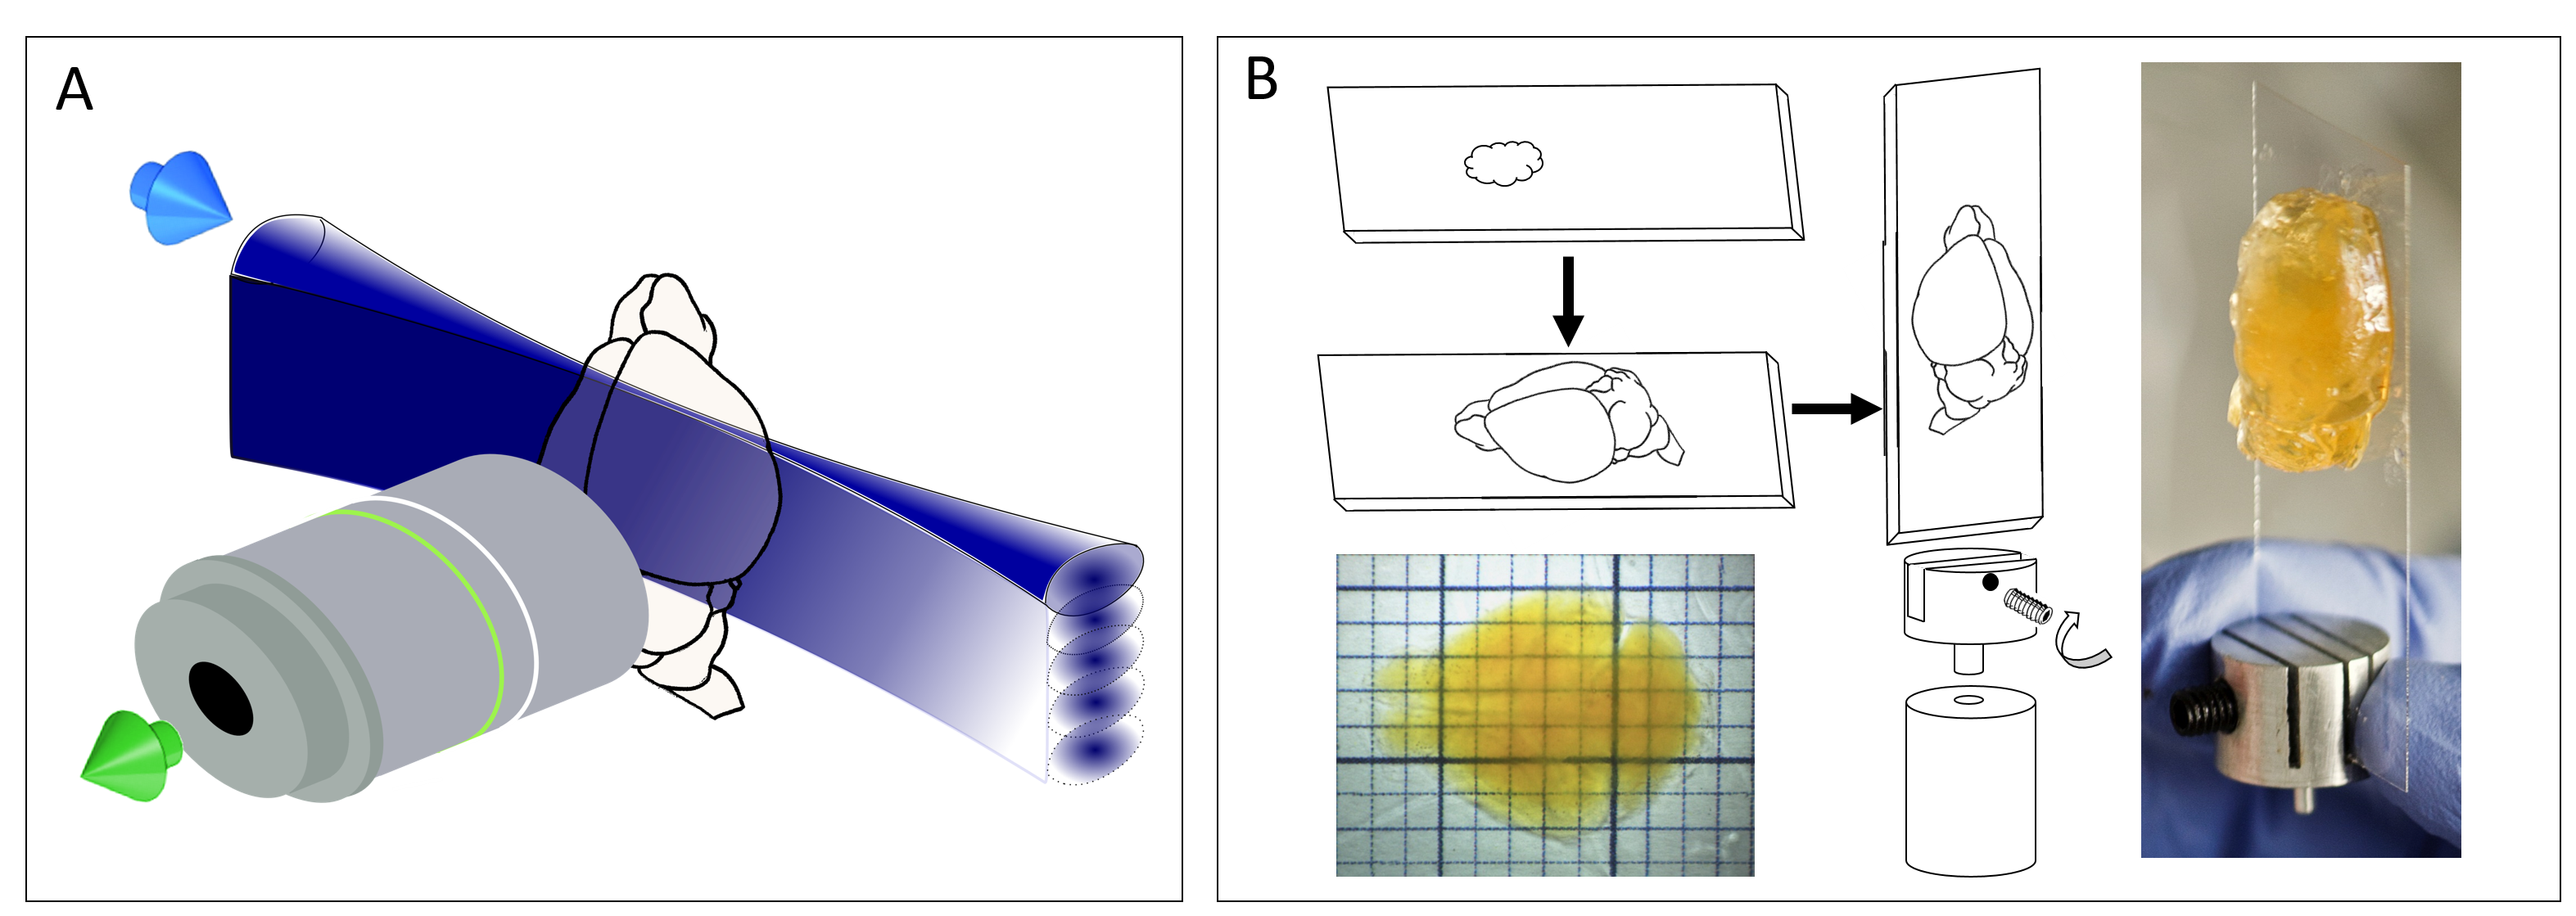
\includegraphics[width=\textwidth]{PanelSampel.eps}
   %\end{tabular}
   %\end{center}
   %\caption{\label{fig:Panel0} (A) Schematic of light-sheet microscopy. The sample is illuminated with a planar light-sheet (blue) perpendicular to fluorescence detection (green). (B) Mounting of a clarified, fluorescently labelled brain. The brain is glued onto a coverslip and inserted into an adapter that slides into a Teflon cylinder.} 
   %\end{figure}

\section{Optical setup}

		
		\begin{figure}
   \begin{center}
   \begin{tabular}{c}
   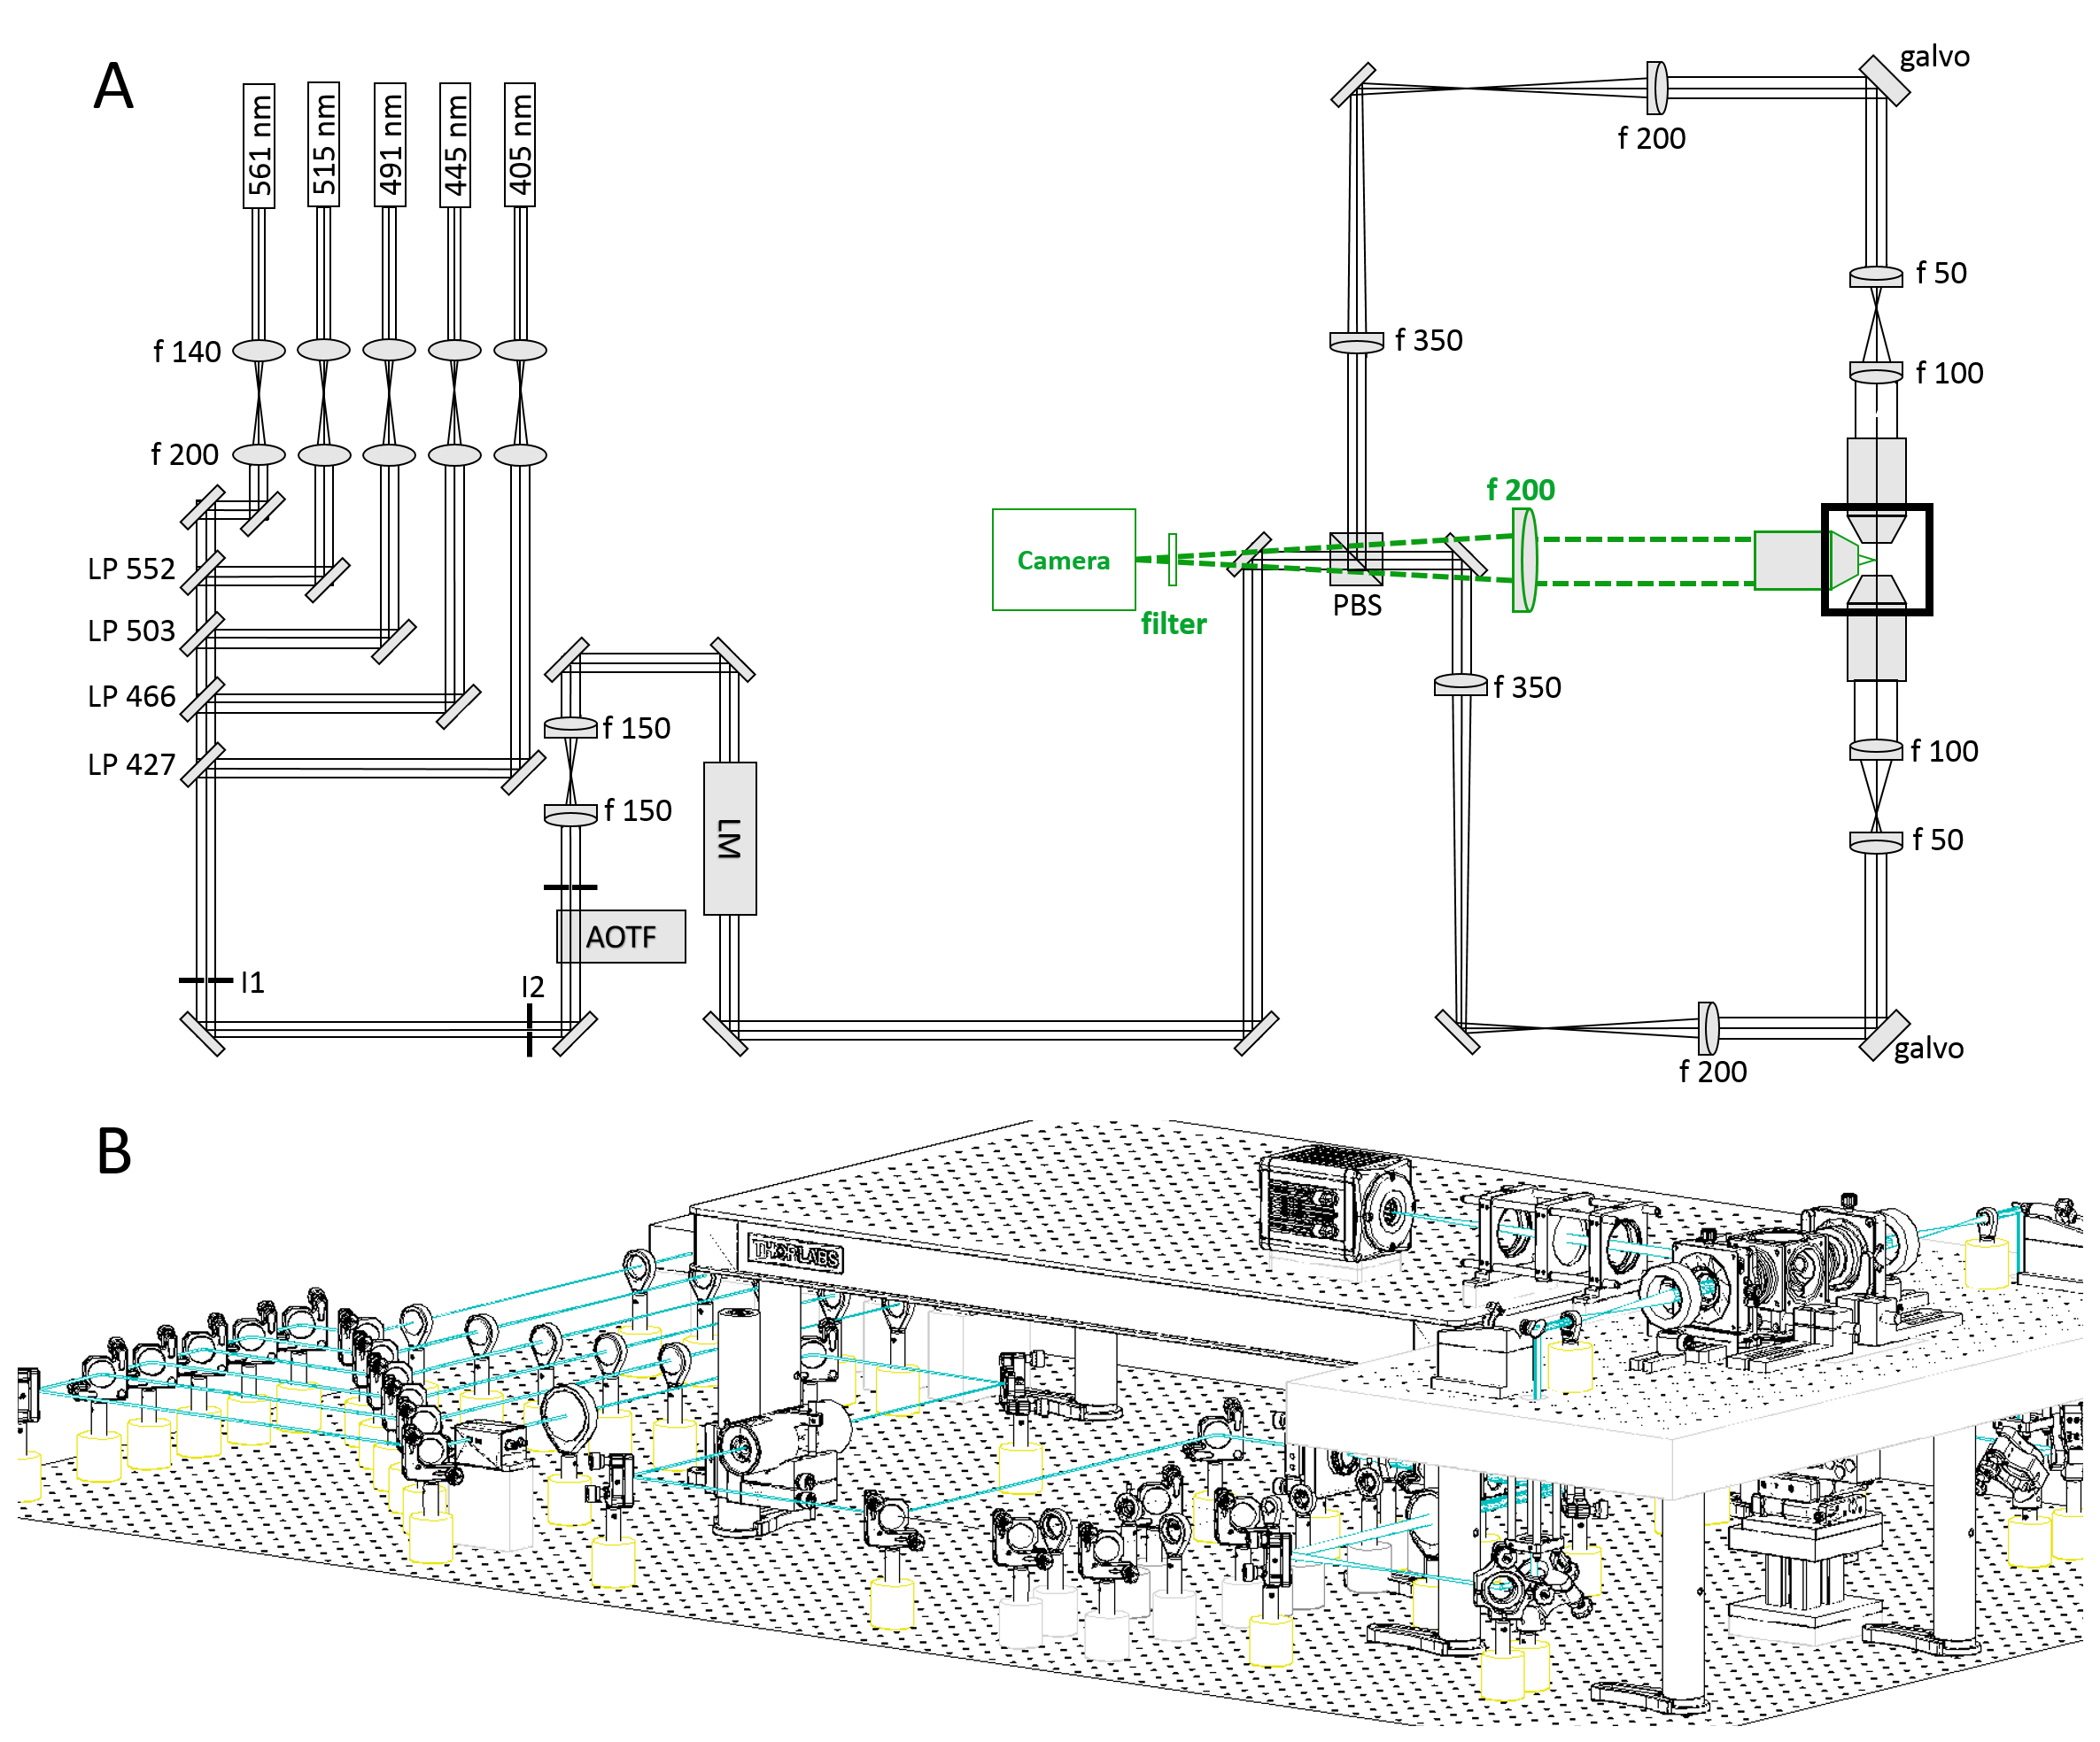
\includegraphics[width=\textwidth]{frame1.eps}
   \end{tabular}
   \end{center}
   \caption{\label{fig:excitation} (A) Topview of the excitation path. The galvo scanners are mounted above periscopes. LP: long-pass filter, I: iris, AOTF: acousto-optical tunable filter, LM: laser modulator, PBS: polarisation beam splitter. Green dotted: detection path. (B) Oblique view of the microscope. A custom-made breadboard serves to mount the sample chamber and objectives at an elevated height and features two circular holes at the edges for the periscopes and a large central cut-out for the translation stages. A second breadboard is used for the camera.} 
   \end{figure}

\subsection{Laser unit}		
The custom-made confocal light-sheet microscope is equipped with 5 linearly polarised cw lasers for fluorescence excitation (Fig. \ref{fig:excitation},A). The wavelengths were chosen to excite the most common fluorophores (see Table \ref{tab:optomechanics} for the manufacturer and specifications of opto-mechanical components). The laser light from each laser is first collimated and expanded with a telescope (f140, f200) and then combined into a common path with a beam steering mirror and a long-pass filter (Semrock, LaserMUX\texttrademark\ series). An acousto-optical tunable filter (AOTF) acts as fast ($\mu s$) electronically tunable filter and intensity modulator. %which uses the acousto-optical interaction inside an anisotropic medium to select and transmit any combination of up to four of the laser lines. The radio-frequency applied on the AOTF transducer controls the wavelength being transmitted into the first order and the radio-frequency amplitude allows to adjust the transmitted light intensity. 
Due its nonlinear response we measured the AOTF light transmittance for each wavelength as a function of radio frequency amplitude and determined a look-up table to linearise the output. The zero order light is blocked by an iris. An electro-optical laser modulator (EOM) acts like a wave plate with electronically controlled retardation and rapidly rotates (few hundreds ns) the input polarisation of the excitation light by $90\degree$. %The wavelength-dependent high voltage that needs to be applied to the birefringent crystal inside the modulator to change the optical path length is provided by a two-step amplification system. First, a low voltage analog signal from the data acquisition and generation (DAQ) board is pre-amplified with custom made electronics and then fed into a commercial high voltage amplifier. 
A digital line is used to switch between the voltage levels, allowing control of the frequency with which the polarisation is changed (see also section \ref{sec:timing} on timing). After the laser modulator the excitation beam is further expanded by a factor of two with two achromatic doublets (f100, f200). 

\subsection{Illumination unit}		
The light impinges onto a polarising beam splitter cube which splits the excitation light depending on its polarisation into one of the two identical excitation arms. The beam diameter is reduced with a telescope (f350, f200) whose telecentric plane coincides with the mirrored surface of a galvanometric scanner (galvo). Both galvos are mounted on a custom made optical breadboard which features two circular holes to pass the periscopic beams and a large central cut-out for the sample chamber and motor stages. 

Each scan mirror surface is re-imaged with a telescope (f50, f100) onto the back aperture of a long working distance low magnification objective (Nikon, 10x 0.3NA WD 17.5mm).  The galvos are in planes conjugate with the back focal plane of their respective excitation objective to ensure that a tilt angle of the galvo converts into a lateral translation of the Gaussian beam across the specimen. The two excitation objectives are designed for air immersion but are immersed into the clearing solution (n=1.45) within the sample chamber. A coverslip glued to the front housing edge serves the dual purpose of maintaining the first diffractive surface between the front optical element and the air and to protect the front lens elements from the organic solvent. A guide to align objectives to a common focus can be found in the supplementary information. The light-sheet is generated digitally\cite{Keller2008a,Keller2008b} by scanning the excitation beam across the focal plane of the detection objective. This generates incoherent illumination resulting in fewer artefacts. %cite{StelzerNatMeth2014}.
Additionally each line in specimen is illuminated with the same intensity creating a homogeneous light-sheet which is particularly advantageous for the quantitative and qualitative investigation of large samples in their entirety.

\subsection{Detection unit}
			
%In its simplest form, the fluorescence detection unit of a light-sheet microscope is a conventional wide-field microscope: an objective lens, a fluorescent filter and a tube lens form an image on a wide-field detector. 
Fluorescence is collected with an objective that is specifically designed for immersion in clearing solutions. The objective is equipped with a correction collar allowing for immersion in media with refractive indices ranging from 1.41 to 1.52 (Olympus, XLSLPLN25XGMP, 25x, 1.0NA, effective focal length 7.2 mm). %To image the whole volume of interest the objective has a relatively low magnification of 25x and a large working distance of 8mm yet a high numerical aperture (1.0NA) affords high resolution imaging. 
A tube lens of 200mm creates the primary image on a sCMOS camera (Orca Flash4.0, Hamamatsu) with a chip of over 4 megapixels. %In contrast to CCD sensors each pixel of a sCMOS camera sensor has a separate photodetector and amplification unit which means that sCMOS pixels can be read out independently from each other. 
The cell size of the OrcaFlash is $p^2= (6.5\micro m)^2$ over an active area of $r^2= (13.3mm)^2$. With a 200mm tube lens the field of view (FOV) in the sample is $480\micro m$ (see also Table \ref{tab:resolution} for relevant formulas). 

In the camera's rolling shutter data acquisition mode only a subset of adjacent horizontal pixel lines is simultaneously exposed and this active detection region is moved across the image sensor\cite{Baumgart2012}. With the delay between the exposure of two adjacent lines set to the minimum time required to read out a single line ($t_{\text{shutter}}=9.7\micro s$) the entire frame of 2048 horizontal lines is activated within 19.86ms. Setting the line exposure time to $t_{\text{exp}}=0.3ms$ results in $l=\nicefrac{t_{\text{exp}}}{t_{\text{shutter}}}\approx31$  lines being simultaneously exposed at any time. This detection area is swept from the top to the bottom of the chip and acts like a moving, virtual confocal slit corresponding to a width of $s_{\text{object}}=\nicefrac{l p}{M_{\text{eff}}}= 7.2 \micro m $ in the sample space, where $M_{\text{eff}}$ is the effective magnification of the detection objective. With the given values of line exposure and line read out time, the camera acquires images at a frame rate of $\nu = \nicefrac{1}{(\#_{\text{horiz. lines}}*t_{\text{shutter}}+t_{\text{exp}})} \approx 50Hz$. 

The camera was run as master in the internal trigger mode and a synchronisation pulse generated with the exposure of each new line was used as as an output trigger for the DAQ board which was operated as slave. The saw-tooth driving signal for the galvo mirrors was generated by the DAQ and synchronised with the pixel line reset pulses from the camera to achieve confocal line detection\cite{Baumgart2012} (see also section \ref{sec:timing} on synchronisation). %Any deviation from precise synchronisation results in image artefacts and severely degraded image contrast. The confocal resolution can be changed at run-time by changing the user-defined line exposure time and with it the rolling shutter width, that is the number of horizontal pixel lines simultaneously exposed.   
 

\subsection{Sample mounting and motion}
\label{sec:mounting}
%Biological tissue is, bar of very few exemptions like the cornea or zebrafish larvae, highly scattering. Scattering is the deflection of light rays due to the heterogeneous mixture of cells and sub-cellular structures with varying refractive indices. Rayleigh scattering, the nearly isotropic and strongly wavelength dependent scattering of light by particles much smaller than the wavelength of light, and Mie scattering, which occurs on cellular structures such as organelles and other refractive structures which are larger than the wavelength of light, far outweigh absorption and cause most biological tissues to be opaque. In the visible spectrum, the scattering of fluorescence photons is dominant over ballistic fluorescence such that for the imaging of large samples optical clearing methods based on refractive index matching have been employed. These methods involve several chemical sample preparation steps to generate transparent yet structurally and anatomically intact tissue.
%
%A successful optical clearing method not only renders the tissue transparent but also causes neither quenching of protein fluorescence nor tissue distortion and is compatible with repetitive immunostaining. A very promising method called CLARITY\cite{Chung2013,Tomer2014} transforms tissue into a nanoporous, hydrogel-hybridized, lipid-free form. Crucially for high through-put clearing and imaging of large samples, the protocol, however, is ideally also fast, easy and cheap. Our lab therefore development a versatile, simple, rapid and inexpensive clearing method based on a water-soluble agent, 2,2'-thiodiethanol (TDE) which in combination with CLARITY allows for the optical clearing of entire mouse brains or human biopsies. With this protocol (see [cite Irene] for a detailed description) a mouse brain (Figure\ref{fig:Panel1},B) takes 1 month to clear at a costs of \$XY.
		
\begin{figure}
   \begin{center}
   \begin{tabular}{c}
   \includegraphics[width=\textwidth]{frame2.eps}
   \end{tabular}
   \end{center}
   \caption{\label{fig:frame2} Schematic of sample mounting and motion. (A) Fluorescence excitation (along x axis) and detection (along z axis) are operated on independent perpendicular light paths where the excitation light-sheet and the detection focal plane overlap. (B) The custom-made sample chamber is assembled with silicone bellows and seal rings. The clarified fluorescently-labelled brain is mounted on a Teflon cylinder in the centre of the watertight chamber filled with clearing solution (C) and can be translated and rotated freely with piezo motors (D). (E) Mounting of a clarified fluorescently labelled brain. The brain is glued onto a coverslip and inserted into an adapter that slides into the Teflon cylinder.} 
   \end{figure}		

We designed a cubic water-tight sample chamber (Fig. \ref{fig:frame2},A) that allows access from all six sides while maintaining the 3D integrity of large clarified and fluorescently-labelled mouse brains. The sample chamber is tightly bolted  to the optical breadboard while soft connections using silicone bellows allow for adjustive movements of the objectives and free 3D motion of the motor stages (Fig. \ref{fig:frame2},B). All connections are sealed with rubber rings and silicone caulk and additionally tightened with cable binders. In this way the objectives can be refocused and realigned without compromising the watertight seal of the chamber (Fig. \ref{fig:frame2},C). The clarified brains are imaged immersed in clearing solution composed of 63\% TDE in Phosphate buffered saline (PBS) and a refractive index of 1.45. To fill the entire volume of the sample chamber approximately 250ml clearing solution are needed. A motorized x-, y-, z-, $\theta$-stage (Physik Instrumente, see Table \ref{tab:optomechanics}) allows free 3D motion and rotation of a Teflon cylinder which reaches into the centre of the chamber (Fig. \ref{fig:frame2},D). Illumination and detection axes are horizontal while sample rotation occurs around the vertical axis.		
		
To elucidate neuronal projections in structurally intact tissue it is paramount to be able to image centimeter-sized clarified samples, such as mouse brains, with high resolution in whole mount preparation. %While promising clearing protocols are well documented in literature\cite{Chung2013,Tomer2014}, the question of sample preparation and mounting in light-sheet microscopy is not trivial but requires novel approaches to such extent that it is becoming a separate field of research and very diverse strategies such as FEP tubes, 3D printed chambers and Quartz cuvettes have been reported\cite{Kaufmann2012,Pitrone2013,Olarte2012,Tomer2014}, however, these approaches are limited to much smaller sample volumes. 
The problem of sample mounting in a light-sheet microscope arises from the fact that optical access to the sample is required from 3-4 planar sides leaving only two opposing sides to insert, fix and move the sample. %Most commonly the vertical direction is chosen. 
Stable mounting is hereby a key concern as a whole brain tomography can require image acquisition in excess of 24 hours and the effects of gravity, tissue shrinking/expansion and evaporation of the clearing solution over such time spans might have to be considered. 

For the acquisition of whole brain data sets, we fix a clarified and fluorescently-labelled mouse brain with super glue to a coverslip (Fig. \ref{fig:frame2},E). The brain is oriented along its axial orientation with the olfactory bulbs at the top and the cerebellum at the bottom of the coverslip. The coverslip is slid into a bottom adaptor and tightened with a plastic-capped grub screw. The bottom adaptor is inserted into a Teflon cylinder with the coverslip being positioned on the far side of the detection objective. Three different slits in the adapter correspond to varying distances to the detection objective and give variability in sample thickness for example to allow also for the mounting of rat brain hemispheres.
	
\subsection{Optical characterisation}

\subsubsection{Theoretical considerations}

The optical properties of a microscope can be summarised by the point-spread function (PSF), which is the image of a point source in object space. In particular, the radial (i.e. perpendicular to the detection axis) and axial (i.e. parallel to the detection axis) resolution of the microscope can be quantified with the full width at half-maximum (FWHM) of the PSF itself along the chosen direction (see Fig. \ref{fig:origin},A). In a light-sheet microscope axial and radial resolution are determined by the numerical aperture (NA) of the illumination and detection optics respectively. The radial PSF is a standard Airy function whose FWHM is given by:

\begin{equation}
\text{FWHM}_{\text{radial}} \simeq \frac{0.51 \lambda_0}{\text{NA}_{\text{d}}} \, ,
\end{equation}

$\lambda_0$ being the wavelength in vacuum and $\text{NA}_{\text{d}}$ the NA of the detection objective. The axial resolution is dominated by the thickness of the light-sheet which for high NA detection objectives is usually larger than the depth of field of the detection objective. If Gaussian beams are used for illumination, the thickness of the light-sheet can be calculated by the well-known formulas of Gaussian optics\cite{Teich}. The radius of the beam waist is given by:

\begin{equation}
w_0 = \frac{\lambda f_{\text{i}}^{\text{eff}}}{\pi w} \, ,
\end{equation}

where $w$ is the $1/e^2$ radius of the beam entering the illumination objective, $ f_{\text{i}}^{\text{eff}}$ is the effective focal length of the illumination optics and $\lambda$ is the wavelength in the medium ($\lambda = \lambda_0 / n$, $n$ being the refractive index). Note that for air objectives (as the one we use for illumination) the effective focal length is extended by a factor $n$ when used inside a medium with refractive index different from unity\cite{Silvestri2012}.
The axial FWHM is then given by:

\begin{equation}
\text{FWHM}_{\text{axial}} \simeq 1.177 w_0 \, .
\end{equation}

The thickness of the light-sheet is not constant throughout the FOV due to the limited depth of focus of the Gaussian beam. The latter can be quantified by the confocal parameter $b$, which is the distance along which the beam $1/e^2$ radius remains relatively constant and smaller than $\sqrt{2} w_0$:

\begin{equation}
b = \frac{2\pi w_0^2}{\lambda} = \frac{2 \lambda  {(f_{\text{i}}^{\text{eff}})}^2}{\pi w^2}\, .
\end{equation}

The need to have an almost uniform resolution in the camera FOV imposes a lower bound to $b$ and thus (according to the previous equations) a limit to the axial resolution. In our setup we adjusted the telescopes in the excitation path in order to have $w \simeq 0.73 mm$, resulting in $b \simeq 346 \micro m$ (corresponding to 72\% of the FOV) and $\text{FWHM}_{\text{axial}} \simeq 5.13 \micro m$. An overview of the relevant formulas concerning the optical properties of a light-sheet microscope is given in Table \ref{tab:resolution}. The reader is referred to this table as a quick guide to tailor their microscope to their specific needs.

\subsubsection{Experimental characterisation}

\begin{figure}
   \begin{center}
   \begin{tabular}{c}
   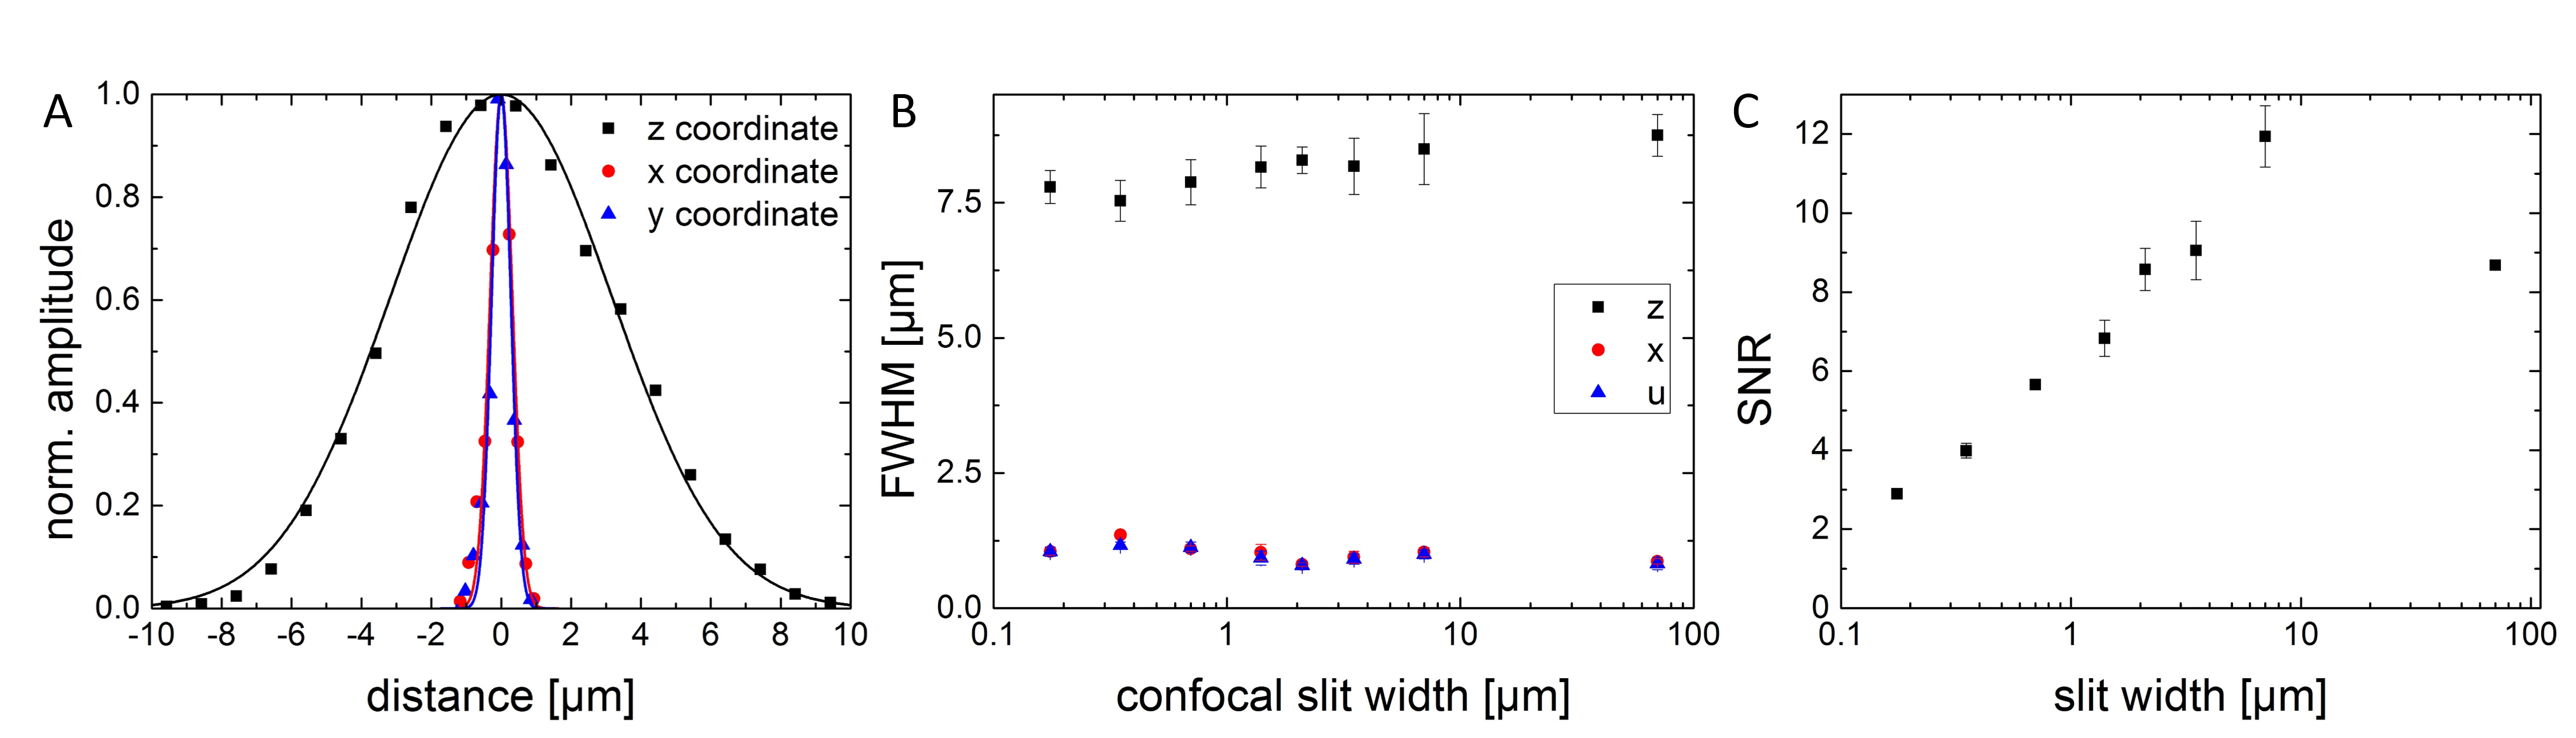
\includegraphics[width=\textwidth]{origin.eps}
   \end{tabular}
   \end{center}
   \caption{\label{fig:origin} Optical characterisation. (A) Exemplary lateral and axial intensity profiles of sub-resolution beads and fits to Gaussian. (B) For each unit 10 bead profiles were fitted in all three dimensions and their FWHM was averaged. (C) The signal to noise ratio.} 
\end{figure}

For optimal imaging it is crucial that the sample-emitted line of fluorescence is in the centre of the rolling shutter at the start of each image acquisition and furthermore travels with the same speed during stack acquisition. To this end the galvo scanners were calibrated using a fluorescein solution in the sample chamber and an image of the focal line was acquired for a set of mirror angles. By fitting each focal line profile to a Gaussian curve the position of the beam main axis was determined and plotted against the voltage applied to the galvo scanner. A linear fit to this data yielded the precise amplitude and offset for each galvo scanner. The finite width of the confocal slit was hereby taken into account such that maximum beam deflection corresponded to the central pixel line of the confocal slit coinciding with the first and last pixel row on the camera chip. From the same data the average FWHM of the Gaussian excitation line over the FOV of the camera was calculated as $(8.60\pm0.67)\micro m$ (n= 14).

For quantitative analysis of spatial resolution and the signal to noise ratio (SNR) we acquired image stacks of nanometric fluorescent beads ($0.51 \micro m$ diameter, Bangs Laboratories). The spatial resolution, in agreement with previous findings\cite{Wilson1987,Cox2004}, was not affected by the confocal slit width on the camera (Fig. \ref{fig:origin},B). The lateral and axial FWHMs were $(1.00\pm0.04) \micro m$ and $(8.13\pm0.14) \micro m$ respectively, averaged through stack depths and confocal slit widths. The experimentally determined lateral FWHM was larger than the theoretically calculated value of $0.26 \micro m$ by a factor of four while the experimentally determined axial FWHM was 1.6x larger than the theoretically calculated value of $5.13 \micro m$. The discrepancies, most notably in the lateral direction, are likely caused by aberrations introduced by the gel embedding the fluorescent beads.

Qualitatively, the SNR increased with increasing slit width up to a maximum around the $1/e^2$ illumination beam diameter of $8.6 \micro m$ and then decreased again with further increasing slit width (Fig. \ref{fig:origin},C) in agreement with previous observations\cite{Baumgart2012}.   



\section{Microscope management software}

\subsection{General design}
The many components of the microscope (camera, lasers, AOTF, stages, etc.) are orchestrated and operated through a custom-made software written in the LabVIEW language (National Instruments, Austin, US). Since the microscope should work mainly without human intervention for many hours (a whole-brain tomography can last a couple of days) without losing precise synchronization, stringent software design is a primary concern. The overall architecture of the software and its practical implementation were chosen to satisfy two main principles; firstly, operation in a distributed environment and secondly, robustness and ease of maintenance. This means, the apparatus should be able to deal with many independent hardware components, and with several data streams (see below). Individual processing steps and/or data transfer can be computationally intensive, and may need to be distributed over several computers to perform properly at run-time. Any kind of hardware problem, from timing delay to real failure, must be automatically handled to avoid loss of data.

%\begin{itemize}
%\item{\emph{User-friendliness}. The light-sheet microscope presented was designed and developed by optical technology specialists yet needs to be operational in a multi-user environment. The greatest challenge therefore consists in making the use of the microscope easy and intuitive such that no formidable proficiency is needed when it is operated by researchers with no expertise in optics and/or software development.}
%\item{\emph{Working in a distributed environment}. The apparatus should deal with many independent hardware components, and with several data streams (see below). Individual processing steps and/or data transfer can be computationally intensive, and may need to be distributed over several computers to perform properly at run-time.}
%\item{\emph{Robustness and ease of maintenance}. Any kind of hardware problem, from timing delay to real failure, must be automatically handled to avoid loss of precious data. Furthermore, developers must be able to fix and expand existing code without having to change the whole software.}
%\item{\emph{Reusability and scalability}. When a second or third microscope with basic similarity yet slightly specialised equipment is being designed in the same or in other laboratories, re-writing all the code from scratch represents extensive but avoidable loss of time. Writing well structured, scalable and easily maintainable scientific software can help preventing redundancy and boosting up productivity.}
%\end{itemize}

%Our microscope management software has been written in LabVIEW (), as this language is particularly well suited for hardware control and data acquisition through pre-developed methods. 
An object-oriented programming framework \cite{castagna1997object} has been used, dividing the entire project into well-defined self-contained modules. This framework, besides helping defining the proper scope of each software component, guarantees robustness, ease of maintenance, scalability and reusability. Code is stored on GitHub (www.github.org) to help multiple users developing software simultaneously. %The graphical user interface (GUI) provides intuitive control of the apparatus as well as full personalisation. In general, the instrument parameters are already set to optimal values stored on disk, and on-line tips on how to set or change the various settings are provided. Both GUIs and code are developed according to the LabVIEW Style Guide \cite{LabviewStyle}.

\subsection{System timing}
\label{sec:timing}

	\begin{figure}
   \begin{center}
   \begin{tabular}{c}
   \includegraphics[width=\textwidth]{connectivity.eps}
   \end{tabular}
   \end{center}
   \caption{\label{fig:connectivity} Schematic view of the hardware architecture of the microscope. Different kind of physical connections are depicted with different colours.} 
   \end{figure}

A schematic overview of the hardware architecture of our light-sheet microscope is shown in Fig. \ref{fig:connectivity}. One personal computer (Precision T5600, Dell, Round Rock, USA, see also Table \ref{tab:optomechanics}) controls all the remote hardware components with the exception of the camera, which is controlled by a second, dedicated computer (Precision T7500, Dell, Round Rock, USA) to handle and manage the enormous streams of data produced (see next section). Various instrumentations are addressed either through computer ports (as USB, RS232 and CameraLink) or via analog and/or digital signals generated by a DAQ board (NI PCIe-6353, National Instruments, Austin, USA).

Synchronization of the camera rolling shutter to the scanning of the light-sheet is achieved by letting the camera acquiring in free-run mode, and using a trigger output from the camera itself to time the generation of the waveforms sent to the galvo drivers. In particular, the HSYNC signal from the camera is used, providing a true-type-logic (TTL) pulse every time the rolling shutter steps from one line to the next one. This trigger signal is used as a clock by the DAQ board, so that the line producing the light-sheet moves step by step with the rolling shutter. The same HSYNC signal is used to trigger the DAQ digital signal sent to the electro-optic laser modulator. In this case, since at each position of the scanning line the modulator should go trough at least two states (vertical polarization and horizontal polarization), HSYNC is used as a trigger while the clock used is the (much faster) internal clock of the DAQ board.




\subsection{Software organisation}
Each hardware component in the microscope (AOTF, galvo scanners, electro-optical modulator, sample stages, camera, lasers) is managed through its own Murmex component (see supplementary information \ref{sec:murmex}). Since the galvo scanners and the electro-optical modulator are not addressed directly, but via analog and digital signals generated by the DAQ board, their software component just sends analog and digital waveforms to an additional intermediate component responsible for DAQ board management. Beyond hardware-related software, two additional Murmex components, the Stack and Tomo components (see below) orchestrate the operation of the entire system. 

The Stack component is used to acquire image stacks along the detection axis, here the $z$ direction, and coordinates the Camera and the Stages components. Stacks are collected by continuously moving the sample along $z$ while keeping the camera acquiring in free run. The translation speed is calculated such that in the time needed to collect a single frame the specimen has moved by a $z$ step specified in the GUI. The Camera component uses low-level libraries from Hamamatsu to save the data, producing one single \emph{.cxd} file (the proprietary, non-compressed, tiff-like format from Hamamatsu) for each image stack. The Camera component must write data to disk with perfect synchronisation, otherwise the nominal $z$ position of each frame is no more coincident with the real $z$ position of the plane imaged. For this reason, we set the process executing the Camera code to be of highest priority. Additionally, the Stack component checks the timing of data production, in order to re-acquire the image stack if the camera has been out-of-time. %The Stack component also specify the name and the path of the \emph{.cxd} file.

The Tomo component is a high level component which coordinates the acquisition of adjacent, parallel, partially-overlapping stacks. %It exchanges messages with the Stack and the Stages components.
The user can specify the volume to be imaged either by inserting the minimum and maximum $x$, $y$ and $z$ coordinates of a parallelepiped or by providing a text file with the coordinates of individual stacks to be collected. The Tomo component informs the experimenter via email when the acquisition is terminated either cleanly or through errors.

All the software described here can be freely downloaded from \href{https://github.com/marcelvanthoff/Giorgio}{GitHub}. Due to its modular structure and of the extensive documentation, it can be easily integrated and adapted in other microscopy systems.

\section{Data Management}
The volume of an adult mouse brain has been estimated from MRI measurements \cite{Kovacevic2005} as $\simeq 0.5$ $\text{cm}^3$; the same authors find out that a parallelepiped encompassing the whole brain would have a volume of $\simeq 0.9$ $\text{cm}^3$. Given the pixel size of the camera and the magnification of the system, and assuming a $z$ step of 2 $\micro$m, the voxel size amounts to $0.234\times0.234\times2$ $\micro\text{m}^3$. This means that a mouse brain will be represented with about 4.6 TeraVoxels, while a parallelepiped encompassing the brain will result in 8.2 TeraVoxels. Since the camera produces 16 bit images with no compression, each raw voxel occupies 2 bytes of disk space, resulting in 8.3 TB for the whole brain "alone" and 14.8 TB for the parallelepiped (see Table \ref{tab:dataproduction}). However, image stacks are acquired with a 10\% of linear superposition, which is later used for image stitching. This redundancy expands the size of raw data to 10.2 TB and 18.3 TB, respectively.

This tremendous amount of data challenges the traditional way we interact with our data. Having far passed the point of taking your data home with you on a hard drive at the end of the experiment, data management in light-sheet microscopy requires the development of a robust data management infrastructure, and of novel software tools to process the images in order to extract meaningful information.

The camera used in our light-sheet microscope (Hamamatsu Orca Flash 4.0 v2) flushes the data stream directly to a dedicated workstation with 12 solid-state drives (SSD) operating in RAID 0 configuration, resulting in a virtual drive of 10.9 TB. Although this is already a large and expensive system for the current SSD technology, it is much smaller than the size of the raw datasets produced in each tomography. We thus connected the workstation to a larger network area storage (NAS) via a 10 Gbit/s network copper cable. The NAS operates in a safer data modality (RAID 5) with 32.4 TB of useful disk space. The NAS is then connected by a dedicated 10 Gbit/s link provided by the Consortium GARR (the Public Institution managing research networks in Italy) to CINECA (the main Italian supercomputing centre). The data flow scheme is summarized in Fig. \ref{fig:DataFlow}.

%Indeed, one stack may consist of thousands of slices of 1024 x 1024 pixels and with a color depth of 16 bits, leading easily to files of tens of Gigabytes each. To efficiently store raw data and make them suited for further processing, we have developed a tool for on-the-fly conversion of files generated during sample acquisitions to multi-page compressed TIFF format.  

While transferring data from the SSD to the NAS, we perform on-the-fly conversion of files generated during sample acquisitions to a multi-page and lossless-compressed TIFF format. %The TIFF format was chosen because it permits storage of a 3D image with lossless compression in a single file. Furthermore, it is a flexible and platform-independent format supported by numerous image processing applications. 
Our conversion module leverages the functionalities offered by the interface of the DCIMGAPI library, supplied by Hamamatsu, and the freely available LibTIFF library. The module reads a single .cxd 3D image and writes it in a variable number of multi-page TIFF files, depending on the user-defined limit of pages per file. Since the output of the Hamamatsu camera may exceed tens of GB, the image in proprietary format is read slice by slice to minimize memory requirements. The conversion module runs concurrently with the microscope controlling software and it synchronizes to convert stack files as soon as they are completed. The module provides options to downsample the image or to save the input image at full or reduced resolution in order to adapt to storage requirements. Usually we downsample the image in the XY plane by a factor 2 and leave the Z sampling unaltered. This downsampling, in combination with the lossless compression offered by the TIFF format, reduces data size by about one order of magnitude. Thus the parallelepiped volume containing the whole mouse brain can be represented using about 2-3 TB of disk space. 

The process executing the file conversion code is set to low execution priority to prevent interference with the Camera component, which needs to be perfectly timed with acquisition. Thus, although file conversion drastically reduces data size, in the current implementation it is slower than data production. The Camera component flushes data on the SSD with a rate $R_{\text{data}}$ dependent on the frame rate $R_{\text{frame}}$ and on the image size $R_{\text{data}} [\text{Bytes}] = 2\cdot R_{\text{frame}} \cdot \#_{\text{pixels}}$
where the factor of two takes into account the 16 bit grey depth of images. The volumetric imaging rate is given by $R_{\text{volume}} = 0.5 R_{\text{data}} \cdot \text{Voxel size}$.

With a standard image size of $2048\times 2048$ pixels, and $R_{\text{frame}}=44$ Hz, data are produced at a rate $R_{\text{data}}=352$ MB/s $\approx 1.2$ TB/h, which results in a volumetric rate $R_{\text{volume}} \approx 2\times 10^7$ $\micro\text{m}^3/s$ $\approx 0.07$ $\text{cm}^3$/h. The conversion module can empty the SSD with an average rate of about 0.7 TB/h, meaning that the SSD is actually filled up during imaging at a rate of about 0.5 TB/h. Imaging sessions should thus be shorter than 21.8 hours: this limits the maximum amount of raw data being acquired continuously to approximately 25.4 TB. This is well above the disk space needed to image the parallelepiped volume encompassing a whole mouse brain. Larger specimens, as rat brain or portion of human brain, must be imaged in consecutive session until faster strategies for image conversion are devised.

	\begin{figure}
   \begin{center}
   \begin{tabular}{c}
   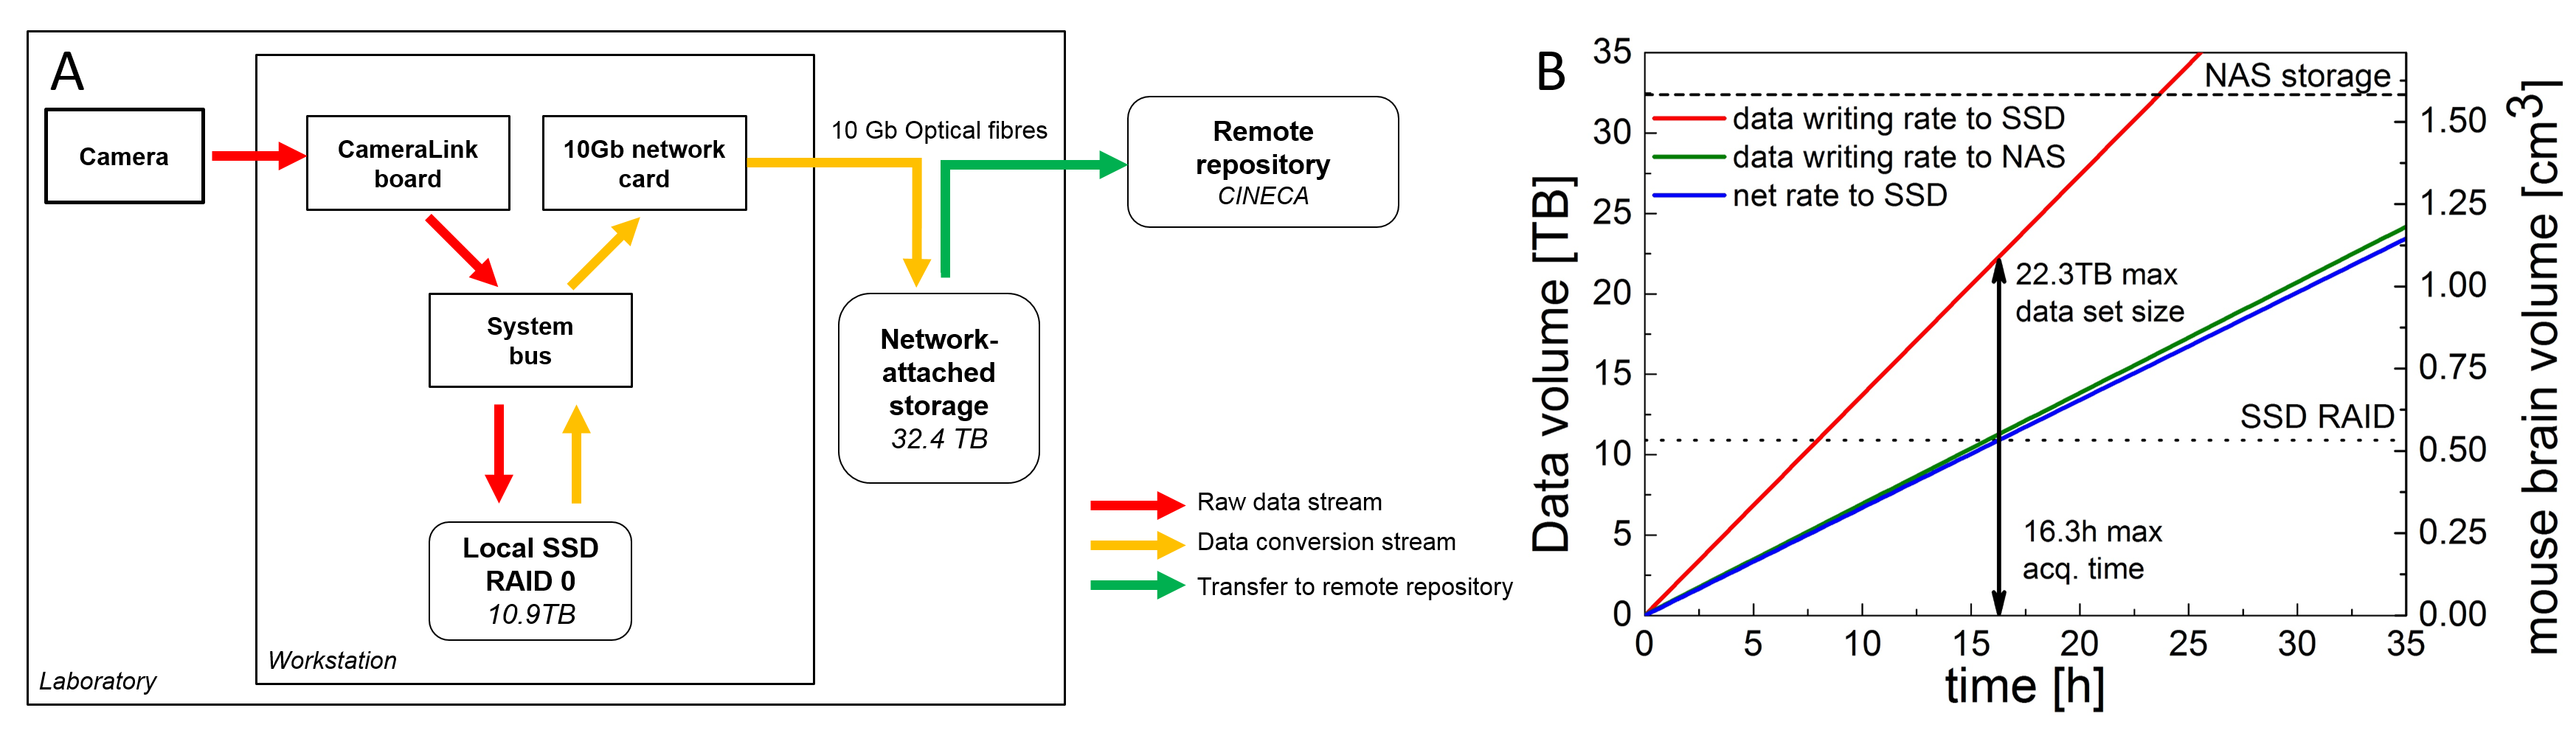
\includegraphics[width=\textwidth]{DataFlow.eps}
   \end{tabular}
   \end{center}
   \caption{\label{fig:DataFlow} Scheme of the data flow. (A) Data streaming on the microscope. SSD: solid-state disk, RAID: redundant array of independent disks, NAS: network-attached storage. Different colours (red, yellow and green) indicate the time-sensitivity (higher to lower) of each data movement. (B) Data production rate versus data conversion rate showing the maximum acquisition time and tomography size feasible before the SSD are filled up.} 
   \end{figure}


\begin{table}%[t!]
	\centering
		\caption[Data production]{Data production rates for typical camera operation.\label{tab:dataproduction}}
		\begin{tabular}{lrl}
		\\
		Voxel size																								& $0.234 \times 0.234 \times 2$	& $\micro\text{m}^3$ 	\\
		Frame rate																								& 44														& Hz								\\
		Frame size																								& $2048 \times 2048$ 						& pixels						\\
		Frame disk size																						& 8									 						& MB								\\
		Data production rate																			& 1.2								 						& TB/h 							\\
		Data conversion rate																			& 0.7								 						& TB/h 							\\
		Net SSD filling rate																			& 0.5								 						& TB/h 							\\
		SSD RAID size																							& 10.9							 						& TB								\\
		Max acquisition time to fill up SSDs											& 21.8							 						& h									\\
		Max raw data size that can be acquired continuously				& 25.4							 						& TB								\\
		Max volume that can be imaged 														& 1.24							 						& $\text{cm}^3$ 		\\
		(considering 10\% superposition between adjacent stacks)	&										 						&										\\
		\end{tabular}
\end{table}

%relevant dimensions in typical acquisition sessions 

After acquisition, the tiled raw image produced has to be stitched. To perform this operation we have used the TeraStitcher\cite{Bria2012}, a fully automated stitching designed to deal with tiled images of virtually unlimited size. TeraStitcher can run on machines with limited resources with a performance essentially determined only by the transfer rate towards secondary storage. TeraStitcher can be freely downloaded from https://github.com/abria/TeraStitcher.

\section{Data}

	\begin{figure}
   \begin{center}
   \begin{tabular}{c}
   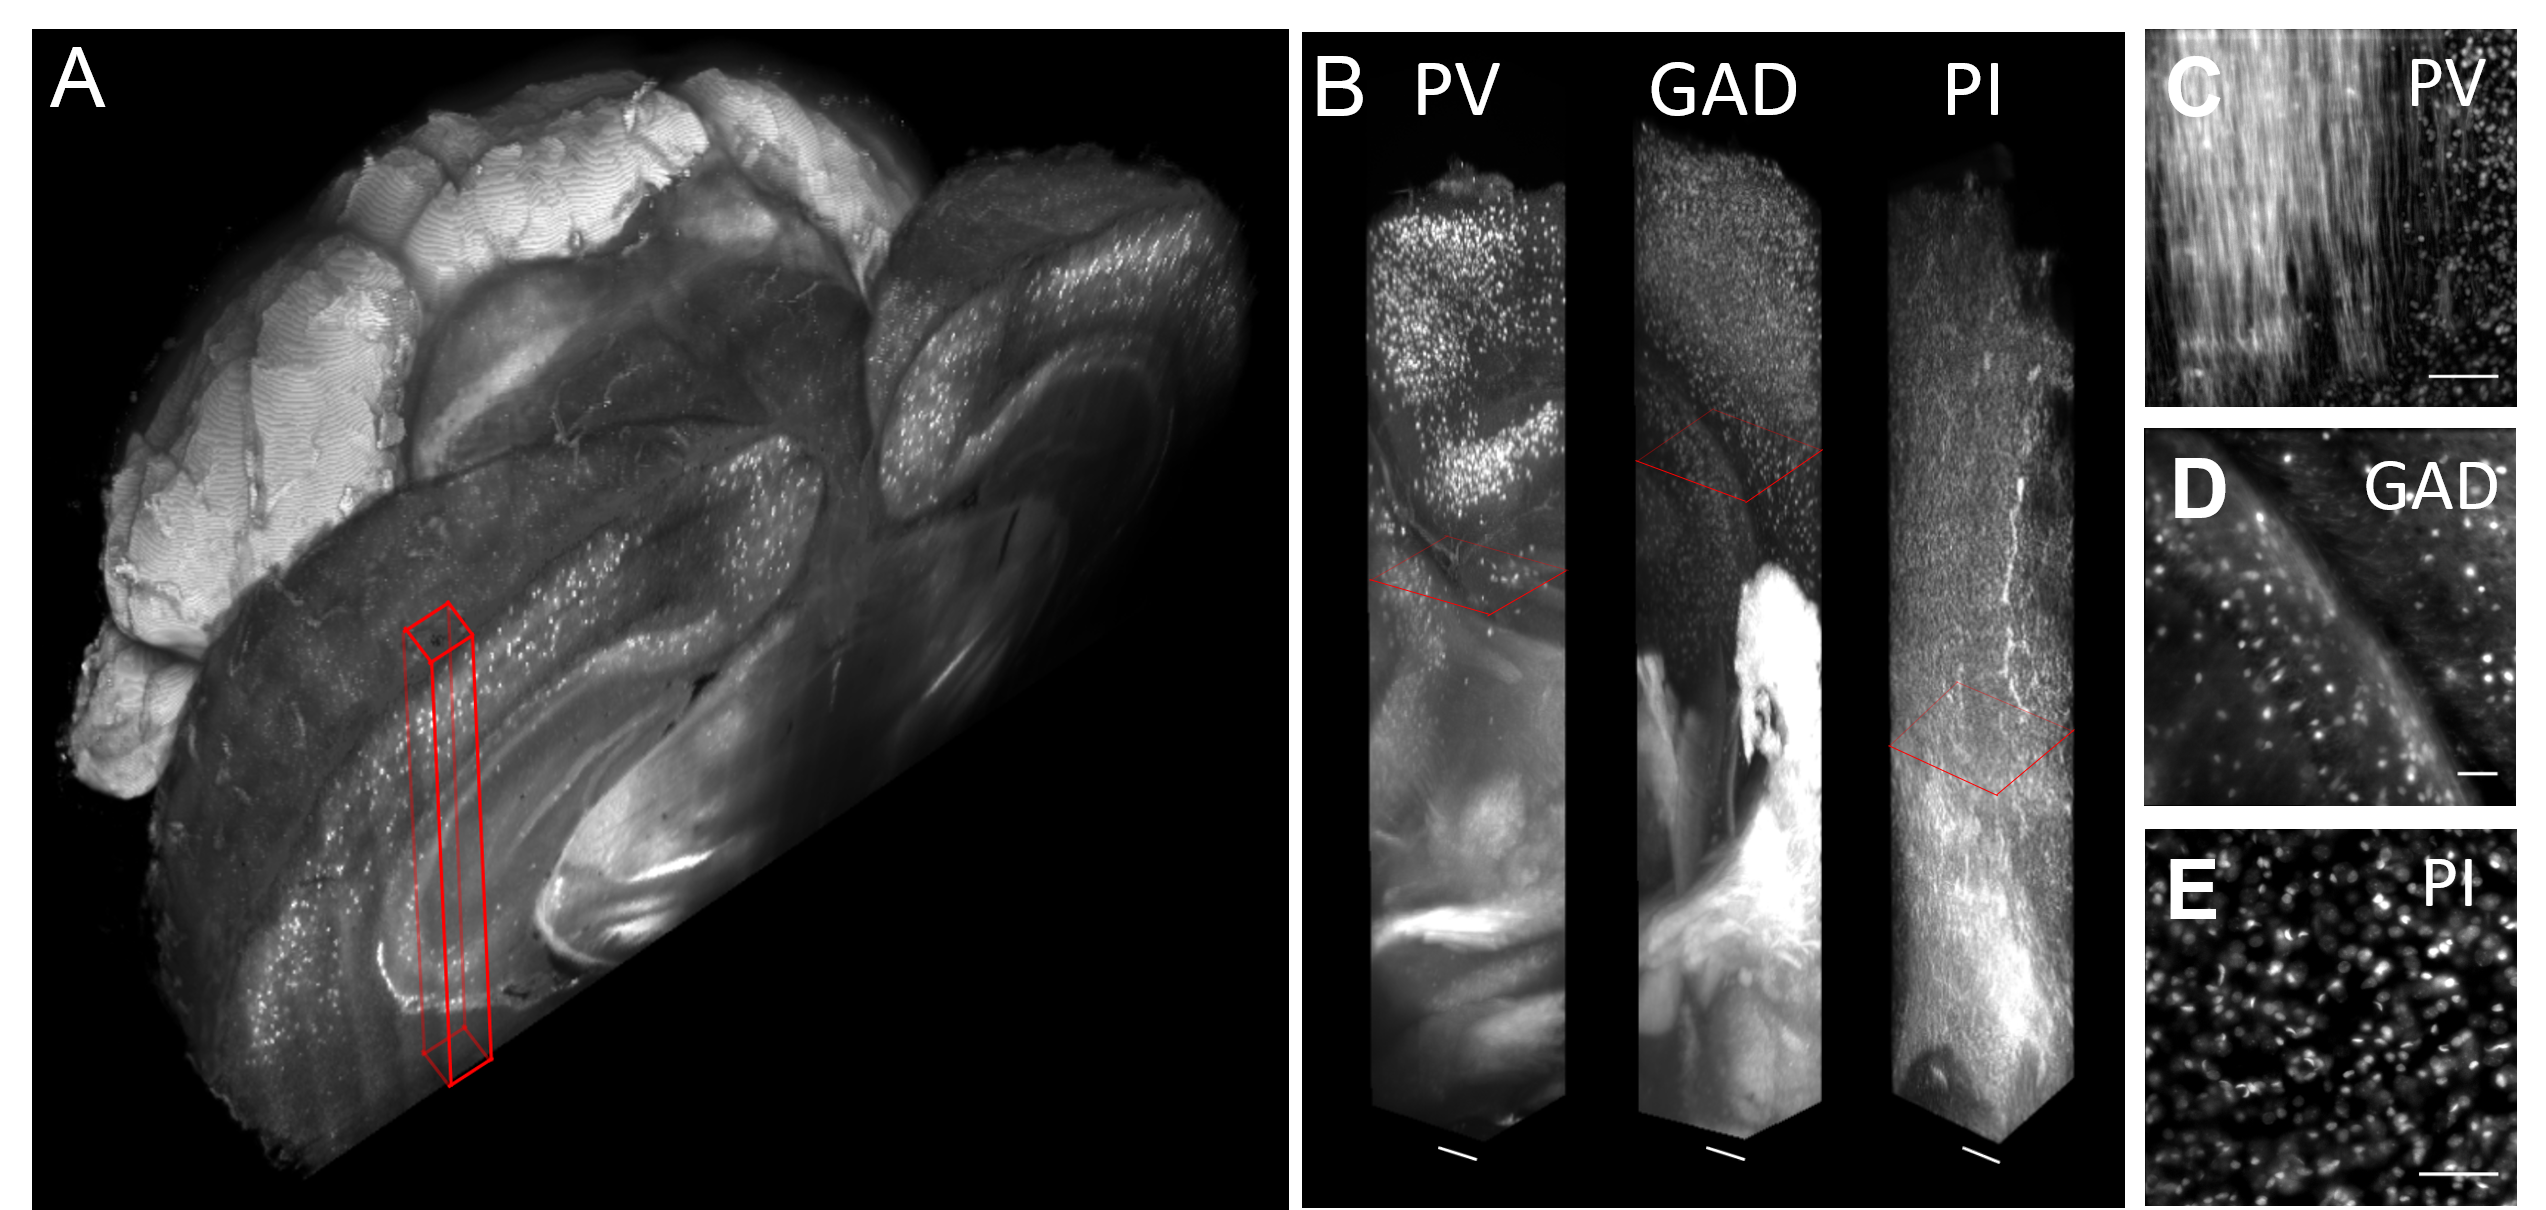
\includegraphics[width=\textwidth]{data_panel.eps}
   \end{tabular}
   \end{center}
   \caption{\label{fig:LSMdata} Whole mouse brain tomography. Imaging of whole transgenic mouse brains treated with CLARITY and cleared with TDE 63\% imaged with Olympus, 25X objective. (A) 3D rendering of a parvalbumin-dTomato brain. (B) 3D rendering of stacks from PV-dTomato mouse brain, GAD-dTomato mouse brain,  PI stained mouse brain, scale bar = $400 \micro m$. (C,D,E) High resolution insert, of the stack corresponding to red boxes in C. Scale bar = $100 \micro m$.} 
   \end{figure}
	
	To exemplify the imaging capabilities of our microscope see Fig. \ref{fig:LSMdata}. 

\section{Conclusion}

%essential features of a good discussion:
%• Try to present the principles, factual relationships and generalisations shown by the results. Discuss dont recapitulate.
%• Noting strengths and limitations. Point out nay exceptions or any lack of correlation and define unsettled points. Never take the high-risk alternative of trying to cover up or fudge data that do not quite fit.
%• Show how your results and interpretations agree (or contrast) with previously published work.
%• Significance of the work: ..so what? Don’t be shy, discuss the theoretical implimication of your work, as well as any possible practical applications. The discussion should end with a short summary or conclusion regarding the significance of the work. Leave with a bang not a whimper.
%• State your conclusions as clearly as possible.
%• Summarise your evidence for each conclusion. Never assume anything.
%• Introduction and discussion function as a pair: the intro should have posed one or more questions. The discussion should indicate what the findings say about the answers. Be sure the discussion answers what the intro asked.
%• Reverse funnel structure: first restate the main findings, then discuss how they relate to findings in previous research, then note implications and applications, and then identify unanswered questions well suited for future research.


Light sheet microscopy has already been a game changer for large-scale, high-throughput imaging by yielding data with a high spatio-temporal scale. The impact of this measurement technique will continue to have a high impact in the field of whole brain imaging due to its ability to record millions of images over the course of days or even weeks. Here we have presented a complete and detailed framework for whole mouse brain imaging. Starting with a full description of our double-sided light sheet microscope and its constituent components we further gave details of the custom-written control software which coordinates the microscope's reliably synchronised operation. The data produced in our experiments easily amounts several TB per data set and needs to be compressed, stored, transferred, retrieved, processed and visualised necessitating the concurrent development of novel computational interface and analysis methods. Here we have presented a comprehensive, robust and fully automated pipeline of data management starting from the streaming of raw images up to the stitching of 3D data sets.

%clearing
The mouse brains imaged in our microscope are intrinsically opaque and need to be clarified before imaging. A successful optical clearing method not only renders the tissue transparent but also causes neither quenching of protein fluorescence nor tissue distortion and is compatible with repetitive immunostaining. A very promising method called CLARITY\cite{Chung2013,Tomer2014} transforms tissue into a nanoporous, hydrogel-hybridized, lipid-free form. Crucially for the high-throughput imaging of large samples that we aim for the protocol, however, is also fast, easy and cheap. We therefore development a versatile, simple, rapid and inexpensive clearing method described elsewhere\cite{Costantini} which in combination with CLARITY allows for the optical clearing of entire mouse brains or human biopsies.

%ao
We have noticed that significant aberrations degrade image quality, especially at depths towards the end of the stack, even in refractive index-matched samples. Recently objectives specifically conceived for LSFM have become commercially available\cite{Marx2014} which have been designed for use with clearing solutions and typically also feature a correction collar for the compensation of a certain amount of spherical aberration. A complete correction of system-induced aberrations, however, requires the ability to also correct for residual spherical aberration and higher-order aberrations introduced by the sample mount, immersion medium and slight misalignments of the optical system. Additionally aberrations introduced by the sample itself degrade image quality. Additionally another problem inherent to light sheet microscopy degrades image quality: due to the uncoupled nature of excitation and detection in LSFM, the aberrations encountered in each arm are independent too and this can lead to a walk-off between the light-sheet and the detection FOV when large samples are imaged at depths. Adaptive optics\cite{Booth2007} provides a means to compensate for these aberrations and has recently been applied to improve LSFM\cite{Jorand2012,Wang2014}. The prospect of high quality images is especially essential for high through-put imaging methods like light-sheet microscopy and whole brain 3D reconstruction because the size of data sets are so large they warrant fully automated post processing for example for automated cell counting and identification\cite{Frasconi2014}. The effect of optical aberrations can severely obscure features even above the resolution limit and therefore hinder automated segmentation of the data. We have mounted the camera on a separate breadboard which leaves us with a lot of free infinity-corrected space in the detection path. In a future paper we aim to implement adaptive optics technology into the fluorescence emission path of our LSFM in order to demonstrate aberration corrected images for whole brain reconstructions. 

%Bessel beam
Further improvements in image quality may be achieved with beam shaping in the illumination arm, for example by implementing Bessel beam illumination\cite{Fahrbach2010,Planchon2011,Gao2014}. Using these self-reconstructing, non-diffractive beams the optical sectioning capability can be improved over an extended field of view.









\begin{landscape}
\begin{table}[t!]
	\centering
		\caption[Components]{Overview of microscope components.\label{tab:optomechanics}}
		\begin{tabular}{llll}
		Component														&	Manufacturer																& Part\# 						& Specifications 														\\\hline\hline
		\multirow{5}{*}[2.5em]{Lasers} 			& \multirow{5}{*}[2.5em]{Cobolt AB, Sweden}		& MLD								& 405nm,  80mW, s-polarised											\\
																				&																							& MLD								& 445nm, 50mW, s-polarised											\\
																				&   																					& Calypso						& 491nm, 50mW, s-polarised											\\
																				&																							& Fandango					& 515nm, 50mW, s-polarised											\\
																				&																							& Jive							& 561nm, 50mW, s-polarised											\\\hline
		AOTF																& AA Opto-Electronic, France									&AOTFnC-400.650-TN 	&	\pbox[t]{10.5cm}{$>90\%$ diffraction efficiency, 3nm resolution, low cross talk between laser lines, high separation angle}\\\hline
		Laser modulator 										& Qioptiq	GmbH, Germany												& LM 0202 VIS ADP		& 400-650nm , $\nicefrac{\lambda}{2}$-voltage (633nm): 210V			\\\hline
		Pulse amplifier 										& Falco Systems, The Netherlands							& WMA-300						& 50x amplification up to $\pm$ 150V, DC to 5MHz signal bandwidth		\\\hline
		Galvo scanner 											& Cambridge Technology, USA										& 6220H 						& small angle step response $200\mu s$								\\\hline		
		\multirow{2}{*}[0.6em]{Objectives}	&	Nikon; Japan																& Plan Fluor EPI 		& 10x0.3NA, WD 17.5mm, EFL 20mm (excitation)						\\
																				& Olympus, Japan															& LMPLFLN20X 				& 20x0.4NA, WD 12mm, EFL 9mm (detection)							\\\hline
		\multirow{3}{*}[1.2em]{Motor stages}& \multirow{2}{*}[0.6em]{Physik Instrumente, Germany}& C-863.11		& DC servo-motor controller								\\
																				&																							&	M-122							& Travel range 25mm, $0.1\micro m$ resolution, max. velocity 20mm/s	\\
																				&																							& M-116 						& Precision Rotation Stage, $2.5\micro rad$, max. velocity $20\degree /s$ \\\hline
		Camera 															& Hamamatsu, Japan														& Orca Flash4.0 	V2.0	& \pbox[t]{10.5cm}{sCMOS sensor, 2048(H) x 2048(V), cell dim.: $6.5\micro m$, active area: 13.3mm x 13.3mm, 16bit images}\\\hline
		DAQ board														& National Instruments, USA										& NI PCIe-6353			& \pbox[t]{10.5cm}{AI: 1 MS/s multichannel; 16-bit resolution, ±10 V; AO: 2.86 MS/s, 16-bit resolution, ±10 V; digital I/O lines (hardware-timed up to 10 MHz), 100MHz max counter frequency}\\\hline
		Workstation 1												& Dell, USA																		& T7500							&  \pbox[t]{10.5cm}{12GB RAM, Intel Xeon Processor X5647 @ 2.93 GHz, OS Windows 7 64 bit}\\
		Workstation 2												& Dell, USA																		& T5600							&  \pbox[t]{10.5cm}{8GB RAM, Intel Xeon Processor E5-2620 @ 2 GHz, OS Windows 7 64 bit}\\
		\end{tabular}
\end{table}
\end{landscape}



%%%%%%%%%%%%%%%%%%%%%%%%%%%%%%%%%%%%%%%%%%%%%%%%%%%%%%%%%%%%%
\acknowledgments
The authors are grateful to Riccardo Ballerini and Ahmed Hajeb from the mechanics workshop at LENS for the conception and fabrication of the sample chamber. We further thank Marco De Pas from the electronic workshop for his expertise in the fabrication of the custom-made amplification electronics. We thank GARR for the 10GB optical fibre connection to CINECA and  CINECA for hosting us on PICO. Human Brain Project tutta la vita and also Ludo's long sentence copy pasta.

\section*{Conflict of interest}
M.v.H has a financial interest in Murmex, Distrio, Amsterdam the Netherlands.


%%%%%%%%%%%%%%%%%%%%%%%%%%%%%%%%%%%%%%%%%%%%%%%%%%%%%%%%%%%%%
%%%%% References %%%%%

%\bibliography{report2}   %>>>> bibliography data in report.bib
\bibliographystyle{spiejour}   %>>>> makes bibtex use spiejour.bst
\begin{thebibliography}{0}

\bibitem{Huisken2009} J. Huisken and D. Y. Stainier, ``Selective plane illumination microscopy techniques in developmental biology," \emph{Development} \textbf{136}(12), 1963–1975 (2009).

\bibitem{Keller2008a} P. J. Keller and E. H. K. Stelzer, ``Quantitative in vivo imaging of entire embryos with digital scanned laser light-sheet fluorescence microscopy," \emph{urr. Opin. Neurobiol.} \textbf{18}(6), 624–632 (2008).

\bibitem{Keller2008b} P. J. Keller, A. D. Schmidt, J. Wittbrodt, and E. H. K. Stelzer, ``Reconstruction of zebrafish early embryonic development by scanned light-sheet microscopy," \emph{Sciences} \textbf{322}(5904), 1065–1069 (20108).

\bibitem{Baumgart2012} E. Baumgart and U. Kubitscheck, ``Scanned light-sheet microscopy with confocal slit detection," \emph{Optics express} \textbf{20}(19), 21805-21814 (2012).

%\bibitem{Kaufmann2012} A. Kaufmann, M. Mickoleit, M. Weber and J. Huisken, ``Multilayer mounting enables long-term imaging of zebrafish development in a light-sheet microscope," \emph{Development} \textbf{139}(17), 3242-3247 (2012).
%
%\bibitem{Pitrone2013} P. Pitrone, J. Schindelin, L. Stuyvenberg, S. Preibisch, M. Weber, K. W. Eliceiri, J. Huisken and P. Tomancak, ``OpenSPIM-an open access platform for light-sheet microscopy," \emph{arXiv} reprint arXiv:1302.1987, 3242-3247 (2013).
%
%\bibitem{Olarte2012} O. E. Olarte, J. Licea-Rodriguez, J. A. Palero, E. J. Gualda, D. Artigas, J. Mayer and P. Loza-Alvarez, ``Image formation by linear and nonlinear digital scanned light-sheet fluorescence microscopy with Gaussian and Bessel beam profiles," \emph{Biomedical optics express} \textbf{3}(7), 1492-1505 (2012).

\bibitem{Teich} M. C. Teich and B. E. A. Saleh, ``Fundamentals of photonics," \emph{Canada, Wiley Interscience} 3 (1991).

\bibitem{Silvestri2012} L. Silvestri, A. Bria, L. Sacconi, G. Iannello,  and F. S. Pavone,  ``Confocal light-sheet microscopy: micron-scale neuroanatomy of the entire mouse brain," \emph{Opt Express} \textbf{20}(18), 20582-20598 (2012).

\bibitem{Wilson1987} T. Wilson and A. R. Carlini, ``Size of the detector in confocal imaging systems," \emph{Opt. Lett.} 12(4), 227–229 (1987).

\bibitem{Cox2004} G. Cox and C. J. Sheppard, ``Practical limits of resolution in confocal and non-linear microscopy," \emph{Microsc. Res. Tech.} 63(1), 18–22 (2004).

\bibitem{Booth2001} M. J. Booth and T. Wilson, ``Refractive-index-mismatch induced aberrations in single-photon and two-photon microscopy and the use of aberration correction," \emph{J. Biomed. Opt.} 6(3), 266–272 (2001).

%\bibitem{LabviewStyle} P. A. Blume, \emph{"The LabVIEW Style Book (National Instruments Virtual Instrumentation Series),"} Prentice Hall PTR (2007).

\bibitem{Kovacevic2005} N. Kovacevic, J. T. Henderson, E. Chan, N. Lifshitz, J. Bishop, A. C. Evans, R. M. Henkelman, and X. J. Chen, "A Three-dimensional MRI Atlas of the Mouse Brain with Estimates of the Average and Variability", \emph{Cereb. Cortex} \textbf{15}(5), 639-45 (2005).

\bibitem{Bria2012} A. Bria and G. Iannello,  ``TeraStitcher-A tool for fast automatic 3D-stitching of teravoxel-sized microscopy images,"  \emph{BMC bioinformatics} \textbf{13}(1), 316 (2012).

\bibitem{Chung2013} K. Chung, J. Wallace, S. Y. Kim, S. Kalyanasundaram, A. S. Andalman, T. J. Davidson and K. Deisseroth, ``Structural and molecular interrogation of intact biological systems," \emph{Nature} \textbf{497}(7449), 332–33 (2013).

\bibitem{Tomer2014} R. Tomer, L. Ye, B. Hsueh and K. Deisseroth, ``Advanced CLARITY for rapid and high-resolution imaging of intact tissues," \emph{nature protocols} \textbf{9}(7), 1682-1697 (2014).

\bibitem{Costantini} I. Costantini, J.-P. Ghobril, A. P. Di Giovanna, A. L. Allegra Mascaro, L. Silvestri, M. C. M\"{u}llenbroich, L. Onofri, V. Conti, F. Vanzi, L. Sacconi, R. Guerrini, H. Markram, G. Iannello, and F. S. Pavone, \emph{submitted}.

\bibitem{Marx2014} V. Marx, ``Microscopy: seeing through tissue," \emph{Nat Meth} \textbf{11}(12), 1209–1214 (2014).

\bibitem{Booth2007} M. J. Booth, ``Adaptive optics in microscopy," \emph{Transactions of the Royal Society A} \textbf{365}(1861), 2829-2843 (2007).

\bibitem{Jorand2012} R. Jorand, G. Corre, J. Andilla, A. Maandhui, C. Frongia, V. Lobjois, B. Ducommun, and C. Lorenzo, ``Deep and Clear Optical Imaging of Thick Inhomogeneous Samples," \emph{PLoS ONE} \textbf{7}(4), (2012).

\bibitem{Wang2014} K. Wang, D. E. Milkie, A. Saxena, P. Engerer, T. Misgeld, M. E. Bronner, J. Mumm, and E. Betzig, ``Rapid adaptive optical recovery of optimal resolution over large volumes," \emph{nature methods} 11(6), 625–628, (2014).

\bibitem{Frasconi2014} P. Frasconi, L. Silvestri, P. Soda, R. L. Cortini, F. S. Pavone and G. Iannello, ``Large-scale automated identification of mouse brain cells in confocal light sheet microscopy images," \emph{Bioinformatics} \textbf{30}(17), i587-i593 (2014).

\bibitem {Fahrbach2010} F. Fahrbach and A. Rohrbach, ``A line scanned light-sheet microscope with phase shaped self-reconstructing beams," \emph{Optics Express} \textbf{18}(23), 780–785 (2010).

\bibitem {Planchon2011} T. Planchon, L. Gao, D. Milkie, M. Davidson, J. Galbraith, C. Galbraith, and E. Betzig, ``Rapid three-dimensional isotropic imaging of living cells using Bessel beam plane illumination," \emph{Nature Methods} \textbf{8}(5), 417–423 (2011).

\bibitem {Gao2014} L. Gao, L. Shao, B.-C. Chen, and E. Betzig, ``3D live fluorescence imaging of cellular dynamics using Bessel beam plane illumination microscopy," \emph{Nature Protocols} \textbf{9}(5), 1083–1101 (2014).



\bibitem{castagna1997object} G. Castagna, \emph{``Object-Oriented Programming A Unified Foundation,"} Birkh{\"a}user, Boston (1997).

\end{thebibliography}


%\listoffigures
%pannel1: optical pathway, drawing images from chamber, sample mirror photos
%pannel2: software scheme
%panel3: hardware connection scheme
%panel4: data pipeline, graph data amount/time
%panel5: experiment pipeline
%panel6: images, tomos



%\listoftables
\pagebreak
\section{Supplementary information}

\subsection{Alignment}

\begin{figure}
   \begin{center}
   \begin{tabular}{c}
   \includegraphics[width=\textwidth]{Panel3.eps}
   \end{tabular}
   \end{center}
   \caption{\label{fig:alignment} (A) Basic geometrical optics of a double-sided illumination light-sheet microscope. AD: achromatic doublet, PBS: polarising beam splitter, red: objective back focal planes and conjugated telecentric planes, green: image planes, blue: 4f telecentric lens system, black: alignment irises. (B) Alignment mirror with drilled hole for light transmission, mount for tip adjustment and adaptor for the Teflon tube. (C) With lateral movement the alignment mirror can be placed such that light is transmitted into the opposing excitation arm. (D) The alignment mirror can be rotated to precisely reflect by $90\degree$.} 
   \end{figure}

For light-sheet microscopy it is crucial that excitation and detection occur on perpendicular axes because any deviation from this geometry results in obscured images of reduced resolution and contrast. The objectives need to be perfectly confocal so that the fluorescence that is generated in the swept excitation beam also falls within the detection objective's focal plane. Telecentric imaging, that is the imaging with two lenses which are the sum of their focal lengths apart, a so-called 4f re-imaging system (Fig. \ref{fig:alignment},A), is used to re-image the galvo scanners onto the back apertures of the excitation objectives. In the detection path, the camera chip needs to be positioned in an image plane of the detection objective. Additionally, homogeneous illumination from both sides impose strict symmetry considerations on both illumination arms that have not only to be sufficiently aligned within themselves respectively but function as a pair with recursive dependence. 

Our microscope was aligned with two tools, a shear plate to qualitatively assess collimation and a small mirror that can be mounted inside the sample chamber where the sample would usually be. The 0.5in mirror was first pierced with a drill using a ceramic drill bit to produce a hole roughly in its centre of the approximately the same diameter as the excitation beam inside the sample chamber (Fig. \ref{fig:alignment},B). Using a compact single axis adjustable mirror mount (V50-AX, Newport) attached to the Teflon cylinder inside the chamber allows to to adjust the pitch of the reflection with the mount and the yaw with the rotation stage while at the same time providing a very space efficient mounting for the pierced 0.5in mirror. With this ``sample mirror" three different position can be easily implemented, firstly, back reflection by hitting the reflective surface at $0\degree$, secondly, transmission by laterally displacing the mirror until the light passes through the drilled hole (Fig. \ref{fig:alignment},C), and thirdly, reflection of the light by $90\degree$ by precisely turning the mirror mount by $45\degree$ using the rotation stage (Fig. \ref{fig:alignment},D). 

\begin{figure}
   \begin{center}
   \begin{tabular}{c}
   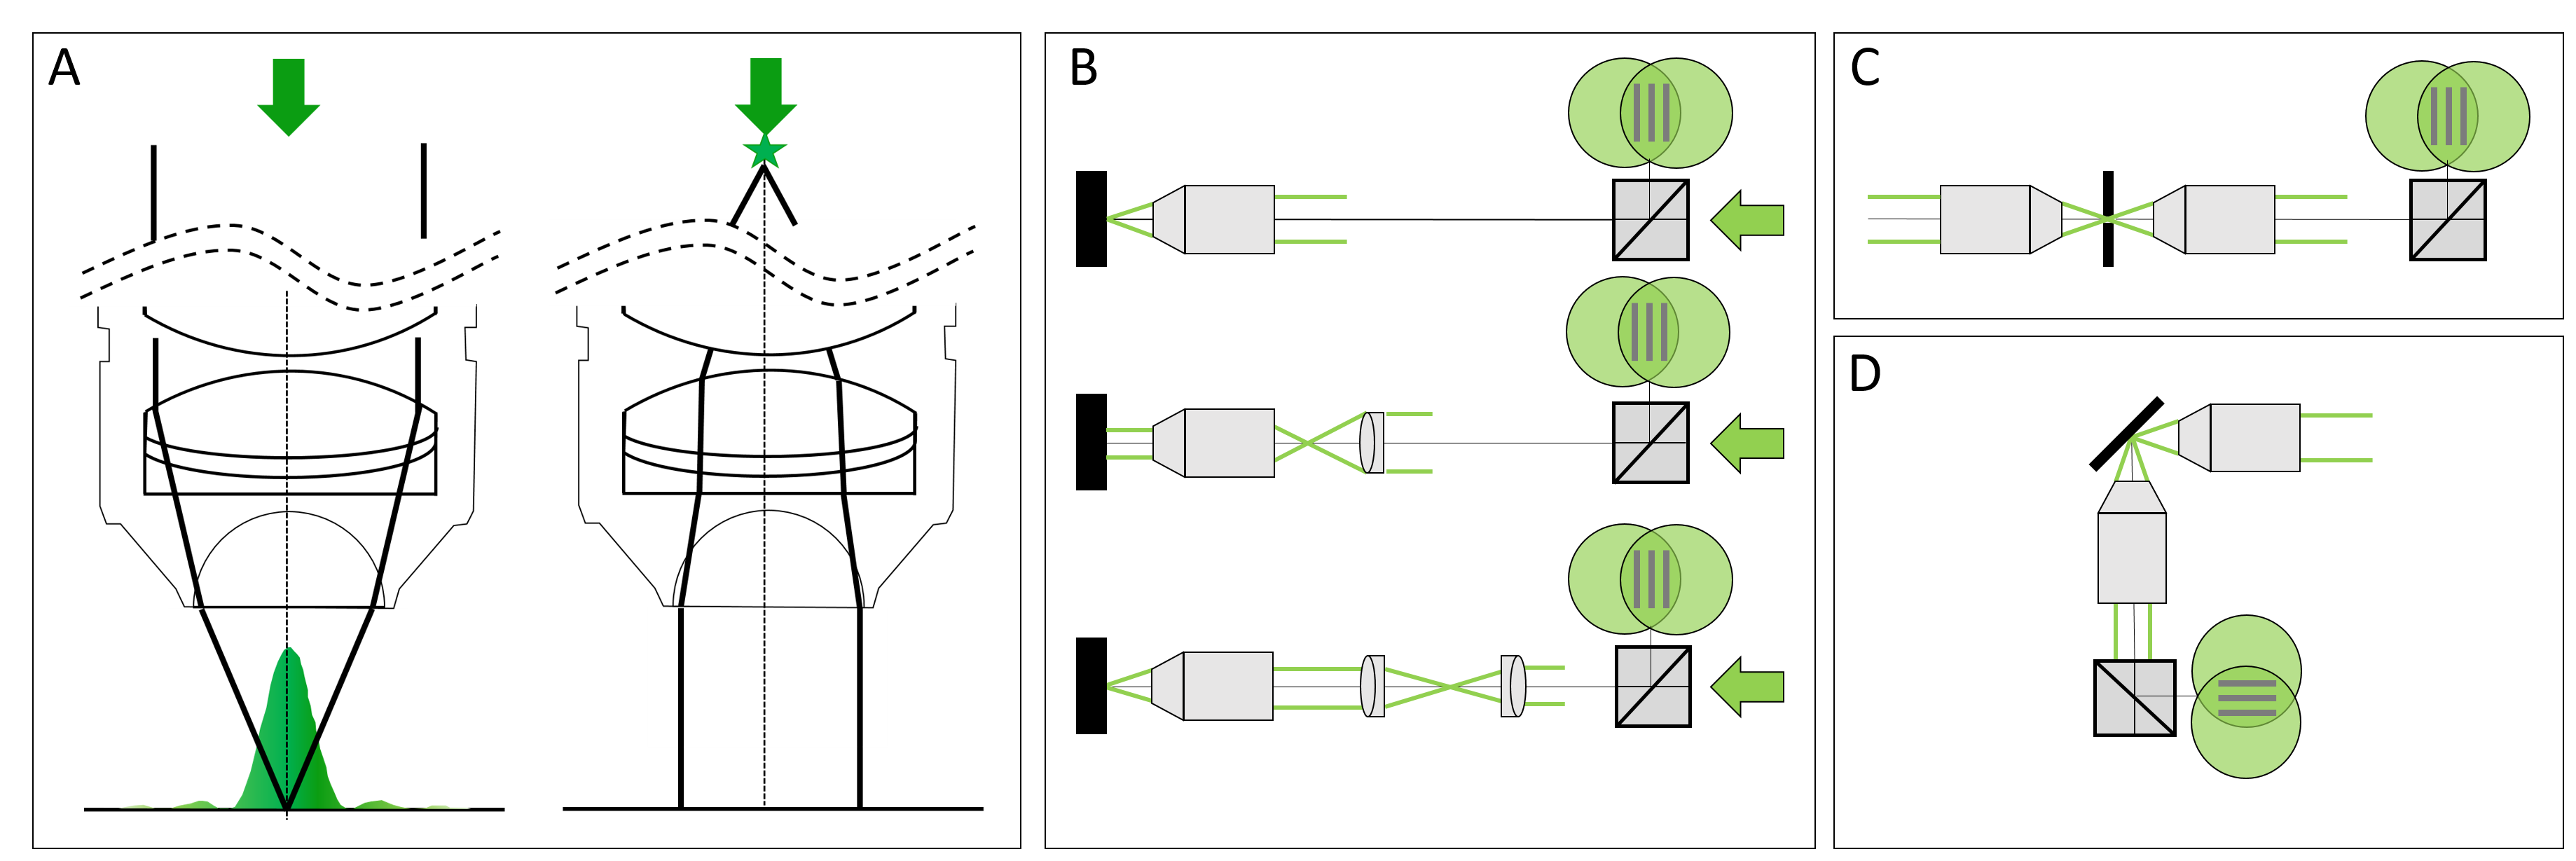
\includegraphics[width=\textwidth]{Panel4.eps}
   \end{tabular}
   \end{center}
   \caption{\label{fig:alignment2} (A) Working principle of a microscope objective (left): a collimated input beam is converted into a spherical wavefront. Right: inverted light path, a focal spot in the back aperture creates a collimated output. (B) Recursive placement of lenses using the sample mirror in back-reflection mode, (C) in transmission mode and (D) in reflection mode.} 
   \end{figure}

The excitation objectives are fixed on mounts which allow three dimensional translation plus pitch and yaw adjustment (LP-1A, Newport). In a first alignment step the beam paths of both excitation arms where brought to overlap through irises placed on the breadboard and the optical bench without any microscope objectives. We found it useful to use two mirrors in each periscope, one vertically mounted and one mounted at $45\degree$ for vertical deflection of the incoming beam. In this way full beam steering can be achieved to realign the periscope before hitting the galvo scanner. After this initial alignment the sample mirror was placed with its reflective surface in the centre of the central cut-out of the breadboard. The first excitation objective was placed into the beam path and brought to focus onto the sample mirror which was adjusted to reflect the light back into the same objective through the irises. Using a shear plate and a beam splitter cube the back reflected light was qualitatively adjusted for collimation using translation along the excitation axis of the objective mount (Fig. \ref{fig:alignment2},B). The sample mirror was then moved laterally to allow the excitation beam to pass through the drilled hole and the second excitation objective was placed (Fig. \ref{fig:alignment2},C). This time collimation was checked with the light going through both objectives and so their confocal placement was insured. Both excitation arms were then aligned recursively by starting at the putative confocal point between the objectives and placing successively lens after lens in the direction towards the light source, alternating between the two modalities illustrated in Fig. \ref{fig:alignment2},A. Finally, the sample mirror was positioned in deflection mode and the detection objective was aligned (Fig. \ref{fig:alignment2},D). 

\subsection{Methods}

\subsubsection{Sample preparation for optical characterisation}
The fluorescent beads (CP01F, Bang Laboratories, $0.51 \micro m$ diameter) used for quantitative analysis of spatial resolution and the signal to noise ratio (SNR) were embedded in low- melting point agarose (2\% agarose in 64\%TDE in PBS). The low melting point agarose (A-4018, Sigma-Aldrich) was dissolved at $40 \degree$ C then mixed with a diluted bead solution and left to polymerise over night on a coverslip. The coverslip was then mounted inside the sample chamber as described in section \ref{sec:mounting}. The embedded sub-diffraction fluorescent beads were imaged with varying confocal slit widths ranging from 0.25 units to 100 confocal units corresponding to slit widths changing from $0.175 \micro m-70 \micro m$ in the sample space. For each slit width one stack of $200\micro m$ depth ($1 \micro m$ step size) was acquired and the one dimensional PSF in the lateral and axial directions were extracted manually with FIJI/ImageJ (eg. Fig. \ref{fig:origin},A) throughout the depth of the image stack. After fitting the lateral and axial profiles with Gaussian curves, the lateral and axial FWHM were averaged (n=10 data points) for different slit widths. The SNR was calculated according to $\text{SNR} = \nicefrac{(y_0 + A)}{y_0}$ where $y_0$ and $A$ are the offset and amplitude of the Gaussian fits.

\subsubsection{Sample preparation for whole brain imaging}



\subsubsection{Murmex}
\label{sec:murmex}
	\begin{figure}
   \begin{center}
   \begin{tabular}{c}
   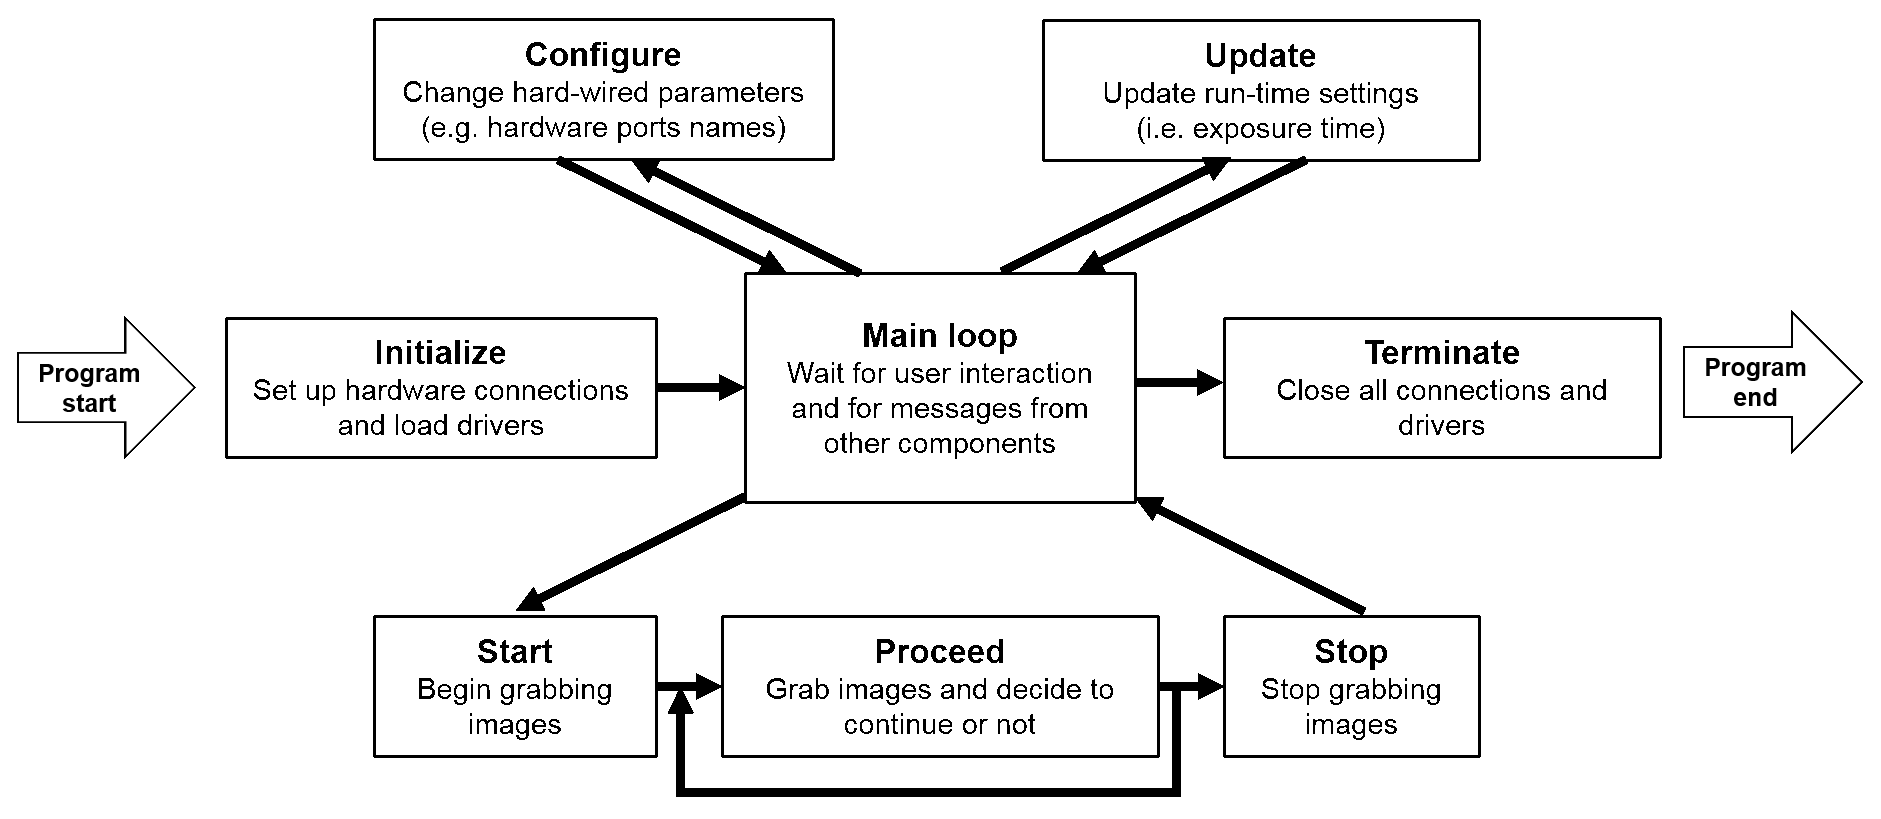
\includegraphics[width=\textwidth]{murmex.eps}
   \end{tabular}
   \end{center}
   \caption{\label{fig:murmex} Schematic view of the work flow of a representative Murmex component operating a camera.} 
   \end{figure}

To operate the software efficiently and synchronously on different machines, the \href{http://sine.ni.com/nips/cds/view/p/lang/en/nid/212895}{Murmex} software development kit was used. This kit integrates the object-oriented programming paradigm with a messaging system, and can be used to create communicating yet independent software modules within a standardized programming scheme.

Murmex creates distributed finite state machines, design patterns in which one component proceeds from a particular state to another based on the message it receives either from itself or from other components. For sending and receiving messages, Murmex uses the library \href{http://sine.ni.com/nips/cds/view/p/lang/en/nid/211065}{LabbitMQ}, which is a wrapper of \href{http://www.rabbitmq.com/}{RabbitMQ}, a message-oriented middle-ware, however, these layers of abstraction are mostly hidden from the developers. %The RabbitMQ server (message broker) needs to be installed either locally or somewhere in the network. 
Buffered, asynchronous and reliable communication between several software components is established by the routing of messages by the broker to the specific software component pinpointed by its ID. %The LabbitMQ wrapper allows use of RabbitMQ inside the LabVIEW programming environment.
Murmex has twelve pre-defined states (eg, Initialise, Configure, Start, Stop, Proceed, Update) and a generic state for implementing custom states. Usually, just a few of this states are actually used in standard application. An example of a standard implementation of the Murmex state machine for the camera is shown in Fig. \ref{fig:murmex}. Each Murmex component streams information about its current status to its 'observers' which are other components specified in its configuration file. Using this oberserver/observee hierarchy, it is possible to design a large and complex network of different components, running on various computers connected through a local connection or the internet while maintaining precise timing and synchronisation. %A special component, named ServiceManager (also based on Murmex), which must be running on each computer, allows to start executables remotely in user-defined compositions of components. This allows the user to start up a sophisticated configuration with multiple components executed on different computers, but operated from one computer.



\subsection{Formulas}

In the table, $f_{\text{TL}}^{\text{design}}$ is the focal length of the tube lens for which the objective has been designed (200 mm for Leica and Nikon, 180 mm for Olympus and 165 mm for Zeiss), $f_{\text{TL}}^{\text{real}}$ the focal length of the tube lens actually employed, $\text{M}$ the nominal magnification of the objective, $n$ the refractive index of the immersion medium, $\lambda_0$ the wavelength in vacuum, $\lambda$ the wavelength in the medium, $w$ the $1/e^2$ radius of the Gaussian beam at the objective back focal plane, FN the field number of the objective, $p$ the physical pixel size, $r_{\text{chip}}$ the size of the camera chip, $t_{\text{shutter}}$ the pace of the rolling shutter (i.e. the time between exposure start in subsequent lines), $ t_{\text{exp}}$ the line exposure time. The subscripts $_i$ and $_d$ refers to illumination and detection, respectively.

\begin{table}[t!]
	\centering
		\caption[Main formulas]{Overview of the main formulas related to light-sheet microscopy. \label{tab:resolution}}
		\begin{tabular}{lrcl}
		\\
		\multicolumn{4}{l}{General formulas for microscope objectives}\\\hline\hline 
		Nominal focal length							& $f$ 													& $=$					& $f_{\text{TL}}^{\text{design}}/\text{M}$				\\	
		Effective focal length						& $f^{\text{eff}}$							& $=$					& $nf$													\\
		Effective magnification						& $\text{M}^{\text{eff}}$				& $=$					& $f_{\text{TL}}^{\text{real}}/f^{\text{eff}}$			\\\\
		\multicolumn{4}{l}{Excitation (Gaussian)}\\\hline\hline	
		Beam waist												&$w_0$													& $=$ 				& $ \lambda f_{\text{i}}^{\text{eff}} / \pi w$				\\
		Axial resolution									&$\text{FWHM}_{\text{axial}}$		& $\approx$   & $ 1.17 w_0 $											\\
		Confocal parameter								& b															& $=$  				& $2 \pi \omega_0^2 / \lambda$							\\
																			&  															& $=$   			& $2 \lambda {(f_{\text{i}}^{\text{eff}})}^2 / \pi w^2 $	\\\\
		\multicolumn{4}{l}{Detection}\\\hline\hline  
		Radial resolution									&$\text{FWHM}_{\text{radial}}$	& $=$					& $0.5 \lambda_0 / \text{NA}_{d}$						\\
		Objective field size							& S															& $=$					& $\text{FN}/{\text{M}}$								\\\\
		\multicolumn{4}{l}{Camera}\\\hline\hline  
		Pixel size object space						& $ p_{\text{object}}$					& $=$					& $p/  \text{M}^{\text{eff}}$							\\
		Camera FOV object space						&$\text{FOV}_{\text{object}}$		& $=$					& $r_{\text{chip}} / \text{M}^{\text{eff}}$				\\
																			&																& $=$					& $p_{\text{object}} \cdot \#_{\text{pixels}}$			\\
		Slit width on camera							& $s_{\text{camera}}$						& $=$					& $ p \cdot t_{\text{exp}} / t_{\text{shutter}} $			\\
		Slit width in object space				& $s_{\text{object}}$						& $=$					& $ s_{\text{camera}}/ \text{M}^{\text{eff}}$			\\
		Frame rate												& $\nu$													& $=$					& $1/(\#_{\text{horiz. lines}} \cdot t_{\text{shutter}} + t_{\text{exp}})$ \\\\

		\end{tabular}
\end{table}

%\end{spacing}
\end{document} 
